
% Default to the notebook output style

    


% Inherit from the specified cell style.




    
\documentclass[11pt]{article}

    
    
    \usepackage[T1]{fontenc}
    % Nicer default font (+ math font) than Computer Modern for most use cases
    \usepackage{mathpazo}

    % Basic figure setup, for now with no caption control since it's done
    % automatically by Pandoc (which extracts ![](path) syntax from Markdown).
    \usepackage{graphicx}
    % We will generate all images so they have a width \maxwidth. This means
    % that they will get their normal width if they fit onto the page, but
    % are scaled down if they would overflow the margins.
    \makeatletter
    \def\maxwidth{\ifdim\Gin@nat@width>\linewidth\linewidth
    \else\Gin@nat@width\fi}
    \makeatother
    \let\Oldincludegraphics\includegraphics
    % Set max figure width to be 80% of text width, for now hardcoded.
    \renewcommand{\includegraphics}[1]{\Oldincludegraphics[width=.8\maxwidth]{#1}}
    % Ensure that by default, figures have no caption (until we provide a
    % proper Figure object with a Caption API and a way to capture that
    % in the conversion process - todo).
    \usepackage{caption}
    \DeclareCaptionLabelFormat{nolabel}{}
    \captionsetup{labelformat=nolabel}

    \usepackage{adjustbox} % Used to constrain images to a maximum size 
    \usepackage{xcolor} % Allow colors to be defined
    \usepackage{enumerate} % Needed for markdown enumerations to work
    \usepackage{geometry} % Used to adjust the document margins
    \usepackage{amsmath} % Equations
    \usepackage{amssymb} % Equations
    \usepackage{textcomp} % defines textquotesingle
    % Hack from http://tex.stackexchange.com/a/47451/13684:
    \AtBeginDocument{%
        \def\PYZsq{\textquotesingle}% Upright quotes in Pygmentized code
    }
    \usepackage{upquote} % Upright quotes for verbatim code
    \usepackage{eurosym} % defines \euro
    \usepackage[mathletters]{ucs} % Extended unicode (utf-8) support
    \usepackage[utf8x]{inputenc} % Allow utf-8 characters in the tex document
    \usepackage{fancyvrb} % verbatim replacement that allows latex
    \usepackage{grffile} % extends the file name processing of package graphics 
                         % to support a larger range 
    % The hyperref package gives us a pdf with properly built
    % internal navigation ('pdf bookmarks' for the table of contents,
    % internal cross-reference links, web links for URLs, etc.)
    \usepackage{hyperref}
    \usepackage{longtable} % longtable support required by pandoc >1.10
    \usepackage{booktabs}  % table support for pandoc > 1.12.2
    \usepackage[inline]{enumitem} % IRkernel/repr support (it uses the enumerate* environment)
    \usepackage[normalem]{ulem} % ulem is needed to support strikethroughs (\sout)
                                % normalem makes italics be italics, not underlines
    

    
    
    % Colors for the hyperref package
    \definecolor{urlcolor}{rgb}{0,.145,.698}
    \definecolor{linkcolor}{rgb}{.71,0.21,0.01}
    \definecolor{citecolor}{rgb}{.12,.54,.11}

    % ANSI colors
    \definecolor{ansi-black}{HTML}{3E424D}
    \definecolor{ansi-black-intense}{HTML}{282C36}
    \definecolor{ansi-red}{HTML}{E75C58}
    \definecolor{ansi-red-intense}{HTML}{B22B31}
    \definecolor{ansi-green}{HTML}{00A250}
    \definecolor{ansi-green-intense}{HTML}{007427}
    \definecolor{ansi-yellow}{HTML}{DDB62B}
    \definecolor{ansi-yellow-intense}{HTML}{B27D12}
    \definecolor{ansi-blue}{HTML}{208FFB}
    \definecolor{ansi-blue-intense}{HTML}{0065CA}
    \definecolor{ansi-magenta}{HTML}{D160C4}
    \definecolor{ansi-magenta-intense}{HTML}{A03196}
    \definecolor{ansi-cyan}{HTML}{60C6C8}
    \definecolor{ansi-cyan-intense}{HTML}{258F8F}
    \definecolor{ansi-white}{HTML}{C5C1B4}
    \definecolor{ansi-white-intense}{HTML}{A1A6B2}

    % commands and environments needed by pandoc snippets
    % extracted from the output of `pandoc -s`
    \providecommand{\tightlist}{%
      \setlength{\itemsep}{0pt}\setlength{\parskip}{0pt}}
    \DefineVerbatimEnvironment{Highlighting}{Verbatim}{commandchars=\\\{\}}
    % Add ',fontsize=\small' for more characters per line
    \newenvironment{Shaded}{}{}
    \newcommand{\KeywordTok}[1]{\textcolor[rgb]{0.00,0.44,0.13}{\textbf{{#1}}}}
    \newcommand{\DataTypeTok}[1]{\textcolor[rgb]{0.56,0.13,0.00}{{#1}}}
    \newcommand{\DecValTok}[1]{\textcolor[rgb]{0.25,0.63,0.44}{{#1}}}
    \newcommand{\BaseNTok}[1]{\textcolor[rgb]{0.25,0.63,0.44}{{#1}}}
    \newcommand{\FloatTok}[1]{\textcolor[rgb]{0.25,0.63,0.44}{{#1}}}
    \newcommand{\CharTok}[1]{\textcolor[rgb]{0.25,0.44,0.63}{{#1}}}
    \newcommand{\StringTok}[1]{\textcolor[rgb]{0.25,0.44,0.63}{{#1}}}
    \newcommand{\CommentTok}[1]{\textcolor[rgb]{0.38,0.63,0.69}{\textit{{#1}}}}
    \newcommand{\OtherTok}[1]{\textcolor[rgb]{0.00,0.44,0.13}{{#1}}}
    \newcommand{\AlertTok}[1]{\textcolor[rgb]{1.00,0.00,0.00}{\textbf{{#1}}}}
    \newcommand{\FunctionTok}[1]{\textcolor[rgb]{0.02,0.16,0.49}{{#1}}}
    \newcommand{\RegionMarkerTok}[1]{{#1}}
    \newcommand{\ErrorTok}[1]{\textcolor[rgb]{1.00,0.00,0.00}{\textbf{{#1}}}}
    \newcommand{\NormalTok}[1]{{#1}}
    
    % Additional commands for more recent versions of Pandoc
    \newcommand{\ConstantTok}[1]{\textcolor[rgb]{0.53,0.00,0.00}{{#1}}}
    \newcommand{\SpecialCharTok}[1]{\textcolor[rgb]{0.25,0.44,0.63}{{#1}}}
    \newcommand{\VerbatimStringTok}[1]{\textcolor[rgb]{0.25,0.44,0.63}{{#1}}}
    \newcommand{\SpecialStringTok}[1]{\textcolor[rgb]{0.73,0.40,0.53}{{#1}}}
    \newcommand{\ImportTok}[1]{{#1}}
    \newcommand{\DocumentationTok}[1]{\textcolor[rgb]{0.73,0.13,0.13}{\textit{{#1}}}}
    \newcommand{\AnnotationTok}[1]{\textcolor[rgb]{0.38,0.63,0.69}{\textbf{\textit{{#1}}}}}
    \newcommand{\CommentVarTok}[1]{\textcolor[rgb]{0.38,0.63,0.69}{\textbf{\textit{{#1}}}}}
    \newcommand{\VariableTok}[1]{\textcolor[rgb]{0.10,0.09,0.49}{{#1}}}
    \newcommand{\ControlFlowTok}[1]{\textcolor[rgb]{0.00,0.44,0.13}{\textbf{{#1}}}}
    \newcommand{\OperatorTok}[1]{\textcolor[rgb]{0.40,0.40,0.40}{{#1}}}
    \newcommand{\BuiltInTok}[1]{{#1}}
    \newcommand{\ExtensionTok}[1]{{#1}}
    \newcommand{\PreprocessorTok}[1]{\textcolor[rgb]{0.74,0.48,0.00}{{#1}}}
    \newcommand{\AttributeTok}[1]{\textcolor[rgb]{0.49,0.56,0.16}{{#1}}}
    \newcommand{\InformationTok}[1]{\textcolor[rgb]{0.38,0.63,0.69}{\textbf{\textit{{#1}}}}}
    \newcommand{\WarningTok}[1]{\textcolor[rgb]{0.38,0.63,0.69}{\textbf{\textit{{#1}}}}}
    
    
    % Define a nice break command that doesn't care if a line doesn't already
    % exist.
    \def\br{\hspace*{\fill} \\* }
    % Math Jax compatability definitions
    \def\gt{>}
    \def\lt{<}
    % Document parameters
    \title{second-conf-call}
    
    
    

    % Pygments definitions
    
\makeatletter
\def\PY@reset{\let\PY@it=\relax \let\PY@bf=\relax%
    \let\PY@ul=\relax \let\PY@tc=\relax%
    \let\PY@bc=\relax \let\PY@ff=\relax}
\def\PY@tok#1{\csname PY@tok@#1\endcsname}
\def\PY@toks#1+{\ifx\relax#1\empty\else%
    \PY@tok{#1}\expandafter\PY@toks\fi}
\def\PY@do#1{\PY@bc{\PY@tc{\PY@ul{%
    \PY@it{\PY@bf{\PY@ff{#1}}}}}}}
\def\PY#1#2{\PY@reset\PY@toks#1+\relax+\PY@do{#2}}

\expandafter\def\csname PY@tok@w\endcsname{\def\PY@tc##1{\textcolor[rgb]{0.73,0.73,0.73}{##1}}}
\expandafter\def\csname PY@tok@c\endcsname{\let\PY@it=\textit\def\PY@tc##1{\textcolor[rgb]{0.25,0.50,0.50}{##1}}}
\expandafter\def\csname PY@tok@cp\endcsname{\def\PY@tc##1{\textcolor[rgb]{0.74,0.48,0.00}{##1}}}
\expandafter\def\csname PY@tok@k\endcsname{\let\PY@bf=\textbf\def\PY@tc##1{\textcolor[rgb]{0.00,0.50,0.00}{##1}}}
\expandafter\def\csname PY@tok@kp\endcsname{\def\PY@tc##1{\textcolor[rgb]{0.00,0.50,0.00}{##1}}}
\expandafter\def\csname PY@tok@kt\endcsname{\def\PY@tc##1{\textcolor[rgb]{0.69,0.00,0.25}{##1}}}
\expandafter\def\csname PY@tok@o\endcsname{\def\PY@tc##1{\textcolor[rgb]{0.40,0.40,0.40}{##1}}}
\expandafter\def\csname PY@tok@ow\endcsname{\let\PY@bf=\textbf\def\PY@tc##1{\textcolor[rgb]{0.67,0.13,1.00}{##1}}}
\expandafter\def\csname PY@tok@nb\endcsname{\def\PY@tc##1{\textcolor[rgb]{0.00,0.50,0.00}{##1}}}
\expandafter\def\csname PY@tok@nf\endcsname{\def\PY@tc##1{\textcolor[rgb]{0.00,0.00,1.00}{##1}}}
\expandafter\def\csname PY@tok@nc\endcsname{\let\PY@bf=\textbf\def\PY@tc##1{\textcolor[rgb]{0.00,0.00,1.00}{##1}}}
\expandafter\def\csname PY@tok@nn\endcsname{\let\PY@bf=\textbf\def\PY@tc##1{\textcolor[rgb]{0.00,0.00,1.00}{##1}}}
\expandafter\def\csname PY@tok@ne\endcsname{\let\PY@bf=\textbf\def\PY@tc##1{\textcolor[rgb]{0.82,0.25,0.23}{##1}}}
\expandafter\def\csname PY@tok@nv\endcsname{\def\PY@tc##1{\textcolor[rgb]{0.10,0.09,0.49}{##1}}}
\expandafter\def\csname PY@tok@no\endcsname{\def\PY@tc##1{\textcolor[rgb]{0.53,0.00,0.00}{##1}}}
\expandafter\def\csname PY@tok@nl\endcsname{\def\PY@tc##1{\textcolor[rgb]{0.63,0.63,0.00}{##1}}}
\expandafter\def\csname PY@tok@ni\endcsname{\let\PY@bf=\textbf\def\PY@tc##1{\textcolor[rgb]{0.60,0.60,0.60}{##1}}}
\expandafter\def\csname PY@tok@na\endcsname{\def\PY@tc##1{\textcolor[rgb]{0.49,0.56,0.16}{##1}}}
\expandafter\def\csname PY@tok@nt\endcsname{\let\PY@bf=\textbf\def\PY@tc##1{\textcolor[rgb]{0.00,0.50,0.00}{##1}}}
\expandafter\def\csname PY@tok@nd\endcsname{\def\PY@tc##1{\textcolor[rgb]{0.67,0.13,1.00}{##1}}}
\expandafter\def\csname PY@tok@s\endcsname{\def\PY@tc##1{\textcolor[rgb]{0.73,0.13,0.13}{##1}}}
\expandafter\def\csname PY@tok@sd\endcsname{\let\PY@it=\textit\def\PY@tc##1{\textcolor[rgb]{0.73,0.13,0.13}{##1}}}
\expandafter\def\csname PY@tok@si\endcsname{\let\PY@bf=\textbf\def\PY@tc##1{\textcolor[rgb]{0.73,0.40,0.53}{##1}}}
\expandafter\def\csname PY@tok@se\endcsname{\let\PY@bf=\textbf\def\PY@tc##1{\textcolor[rgb]{0.73,0.40,0.13}{##1}}}
\expandafter\def\csname PY@tok@sr\endcsname{\def\PY@tc##1{\textcolor[rgb]{0.73,0.40,0.53}{##1}}}
\expandafter\def\csname PY@tok@ss\endcsname{\def\PY@tc##1{\textcolor[rgb]{0.10,0.09,0.49}{##1}}}
\expandafter\def\csname PY@tok@sx\endcsname{\def\PY@tc##1{\textcolor[rgb]{0.00,0.50,0.00}{##1}}}
\expandafter\def\csname PY@tok@m\endcsname{\def\PY@tc##1{\textcolor[rgb]{0.40,0.40,0.40}{##1}}}
\expandafter\def\csname PY@tok@gh\endcsname{\let\PY@bf=\textbf\def\PY@tc##1{\textcolor[rgb]{0.00,0.00,0.50}{##1}}}
\expandafter\def\csname PY@tok@gu\endcsname{\let\PY@bf=\textbf\def\PY@tc##1{\textcolor[rgb]{0.50,0.00,0.50}{##1}}}
\expandafter\def\csname PY@tok@gd\endcsname{\def\PY@tc##1{\textcolor[rgb]{0.63,0.00,0.00}{##1}}}
\expandafter\def\csname PY@tok@gi\endcsname{\def\PY@tc##1{\textcolor[rgb]{0.00,0.63,0.00}{##1}}}
\expandafter\def\csname PY@tok@gr\endcsname{\def\PY@tc##1{\textcolor[rgb]{1.00,0.00,0.00}{##1}}}
\expandafter\def\csname PY@tok@ge\endcsname{\let\PY@it=\textit}
\expandafter\def\csname PY@tok@gs\endcsname{\let\PY@bf=\textbf}
\expandafter\def\csname PY@tok@gp\endcsname{\let\PY@bf=\textbf\def\PY@tc##1{\textcolor[rgb]{0.00,0.00,0.50}{##1}}}
\expandafter\def\csname PY@tok@go\endcsname{\def\PY@tc##1{\textcolor[rgb]{0.53,0.53,0.53}{##1}}}
\expandafter\def\csname PY@tok@gt\endcsname{\def\PY@tc##1{\textcolor[rgb]{0.00,0.27,0.87}{##1}}}
\expandafter\def\csname PY@tok@err\endcsname{\def\PY@bc##1{\setlength{\fboxsep}{0pt}\fcolorbox[rgb]{1.00,0.00,0.00}{1,1,1}{\strut ##1}}}
\expandafter\def\csname PY@tok@kc\endcsname{\let\PY@bf=\textbf\def\PY@tc##1{\textcolor[rgb]{0.00,0.50,0.00}{##1}}}
\expandafter\def\csname PY@tok@kd\endcsname{\let\PY@bf=\textbf\def\PY@tc##1{\textcolor[rgb]{0.00,0.50,0.00}{##1}}}
\expandafter\def\csname PY@tok@kn\endcsname{\let\PY@bf=\textbf\def\PY@tc##1{\textcolor[rgb]{0.00,0.50,0.00}{##1}}}
\expandafter\def\csname PY@tok@kr\endcsname{\let\PY@bf=\textbf\def\PY@tc##1{\textcolor[rgb]{0.00,0.50,0.00}{##1}}}
\expandafter\def\csname PY@tok@bp\endcsname{\def\PY@tc##1{\textcolor[rgb]{0.00,0.50,0.00}{##1}}}
\expandafter\def\csname PY@tok@fm\endcsname{\def\PY@tc##1{\textcolor[rgb]{0.00,0.00,1.00}{##1}}}
\expandafter\def\csname PY@tok@vc\endcsname{\def\PY@tc##1{\textcolor[rgb]{0.10,0.09,0.49}{##1}}}
\expandafter\def\csname PY@tok@vg\endcsname{\def\PY@tc##1{\textcolor[rgb]{0.10,0.09,0.49}{##1}}}
\expandafter\def\csname PY@tok@vi\endcsname{\def\PY@tc##1{\textcolor[rgb]{0.10,0.09,0.49}{##1}}}
\expandafter\def\csname PY@tok@vm\endcsname{\def\PY@tc##1{\textcolor[rgb]{0.10,0.09,0.49}{##1}}}
\expandafter\def\csname PY@tok@sa\endcsname{\def\PY@tc##1{\textcolor[rgb]{0.73,0.13,0.13}{##1}}}
\expandafter\def\csname PY@tok@sb\endcsname{\def\PY@tc##1{\textcolor[rgb]{0.73,0.13,0.13}{##1}}}
\expandafter\def\csname PY@tok@sc\endcsname{\def\PY@tc##1{\textcolor[rgb]{0.73,0.13,0.13}{##1}}}
\expandafter\def\csname PY@tok@dl\endcsname{\def\PY@tc##1{\textcolor[rgb]{0.73,0.13,0.13}{##1}}}
\expandafter\def\csname PY@tok@s2\endcsname{\def\PY@tc##1{\textcolor[rgb]{0.73,0.13,0.13}{##1}}}
\expandafter\def\csname PY@tok@sh\endcsname{\def\PY@tc##1{\textcolor[rgb]{0.73,0.13,0.13}{##1}}}
\expandafter\def\csname PY@tok@s1\endcsname{\def\PY@tc##1{\textcolor[rgb]{0.73,0.13,0.13}{##1}}}
\expandafter\def\csname PY@tok@mb\endcsname{\def\PY@tc##1{\textcolor[rgb]{0.40,0.40,0.40}{##1}}}
\expandafter\def\csname PY@tok@mf\endcsname{\def\PY@tc##1{\textcolor[rgb]{0.40,0.40,0.40}{##1}}}
\expandafter\def\csname PY@tok@mh\endcsname{\def\PY@tc##1{\textcolor[rgb]{0.40,0.40,0.40}{##1}}}
\expandafter\def\csname PY@tok@mi\endcsname{\def\PY@tc##1{\textcolor[rgb]{0.40,0.40,0.40}{##1}}}
\expandafter\def\csname PY@tok@il\endcsname{\def\PY@tc##1{\textcolor[rgb]{0.40,0.40,0.40}{##1}}}
\expandafter\def\csname PY@tok@mo\endcsname{\def\PY@tc##1{\textcolor[rgb]{0.40,0.40,0.40}{##1}}}
\expandafter\def\csname PY@tok@ch\endcsname{\let\PY@it=\textit\def\PY@tc##1{\textcolor[rgb]{0.25,0.50,0.50}{##1}}}
\expandafter\def\csname PY@tok@cm\endcsname{\let\PY@it=\textit\def\PY@tc##1{\textcolor[rgb]{0.25,0.50,0.50}{##1}}}
\expandafter\def\csname PY@tok@cpf\endcsname{\let\PY@it=\textit\def\PY@tc##1{\textcolor[rgb]{0.25,0.50,0.50}{##1}}}
\expandafter\def\csname PY@tok@c1\endcsname{\let\PY@it=\textit\def\PY@tc##1{\textcolor[rgb]{0.25,0.50,0.50}{##1}}}
\expandafter\def\csname PY@tok@cs\endcsname{\let\PY@it=\textit\def\PY@tc##1{\textcolor[rgb]{0.25,0.50,0.50}{##1}}}

\def\PYZbs{\char`\\}
\def\PYZus{\char`\_}
\def\PYZob{\char`\{}
\def\PYZcb{\char`\}}
\def\PYZca{\char`\^}
\def\PYZam{\char`\&}
\def\PYZlt{\char`\<}
\def\PYZgt{\char`\>}
\def\PYZsh{\char`\#}
\def\PYZpc{\char`\%}
\def\PYZdl{\char`\$}
\def\PYZhy{\char`\-}
\def\PYZsq{\char`\'}
\def\PYZdq{\char`\"}
\def\PYZti{\char`\~}
% for compatibility with earlier versions
\def\PYZat{@}
\def\PYZlb{[}
\def\PYZrb{]}
\makeatother


    % Exact colors from NB
    \definecolor{incolor}{rgb}{0.0, 0.0, 0.5}
    \definecolor{outcolor}{rgb}{0.545, 0.0, 0.0}



    
    % Prevent overflowing lines due to hard-to-break entities
    \sloppy 
    % Setup hyperref package
    \hypersetup{
      breaklinks=true,  % so long urls are correctly broken across lines
      colorlinks=true,
      urlcolor=urlcolor,
      linkcolor=linkcolor,
      citecolor=citecolor,
      }
    % Slightly bigger margins than the latex defaults
    
    \geometry{verbose,tmargin=1in,bmargin=1in,lmargin=1in,rmargin=1in}
    
    

    \begin{document}
    
    
    \maketitle
    
    

    
    \section{Joint conf-call report \#2}\label{joint-conf-call-report-2}

    \begin{Verbatim}[commandchars=\\\{\}]
{\color{incolor}In [{\color{incolor}1}]:} \PY{k+kn}{import} \PY{n+nn}{datetime}
        \PY{n+nb}{print}\PY{p}{(}\PY{n+nb}{str}\PY{p}{(}\PY{n}{datetime}\PY{o}{.}\PY{n}{datetime}\PY{o}{.}\PY{n}{today}\PY{p}{(}\PY{p}{)}\PY{p}{)}\PY{p}{)}
\end{Verbatim}


    \begin{Verbatim}[commandchars=\\\{\}]
2018-05-02 12:15:01.378050

    \end{Verbatim}

    \emph{For this second report I am experimenting a new way to fastly
deploy updates about the project: \textbf{Jupyter notebook}. In this
stage of the project, I'd like to share more code snippets than I would
in the final thesis, hence markdown support and live execution of code
snippets turned out to be very useful for such purpose. Actually the two
main reason why I decided to move from raw LaTeX to here are: (1)
Jupyter does it faster, (2) it converts everything to LaTeX (I won't be
required to make any effort to include everything from here to my LaTeX
thesis document). Whether, for any reason, this method will turn out to
be ineffective or time-expensive, then I will drop it out.}

\emph{You will notice changes in style, format and even contents (like
change logs and other stuffs that may appear useless or too much
detailed), this necessity arises since I need to keep track of the
internship's history and I foresee that within few months the commit log
on Github will get a bit messy and too much wide to be relied on,
instead these reports are the easiest way to fulfill such task.}

    \section{Change log summary}\label{change-log-summary}

\subsection{Training set generator
function}\label{training-set-generator-function}

Now domains of all samples' components are centered at the same value
\(c\). Such domains are determined as follows.

Is defined \(K = \{k_1,...k_m\}\) where \(k_i\) is the domain radius of
variable \(x_i\). Let \(x=(x_1,...,x_m) \in X\) be a sample of the
training set, then the domain of \(x_i\) is \(D(x_i) = [c-k_i, c+k_i]\).

\begin{Shaded}
\begin{Highlighting}[]
\KeywordTok{def}\NormalTok{ sample_from_function(n_samples, n_features, func, domain_radius}\OperatorTok{=}\FloatTok{0.5}\NormalTok{, domain_center}\OperatorTok{=}\FloatTok{0.5}\NormalTok{,error_mean}\OperatorTok{=}\DecValTok{0}\NormalTok{, error_std_dev}\OperatorTok{=}\DecValTok{1}\NormalTok{):}
\NormalTok{    X }\OperatorTok{=}\NormalTok{ []}
\NormalTok{    y }\OperatorTok{=}\NormalTok{ np.zeros(n_samples)}
\NormalTok{    w }\OperatorTok{=}\NormalTok{ np.ones(n_features)}
\NormalTok{    K }\OperatorTok{=}\NormalTok{ np.random.uniform(domain_center }\OperatorTok{-}\NormalTok{ domain_radius, domain_center }\OperatorTok{+}\NormalTok{ domain_radius, n_features)}

    \ControlFlowTok{for}\NormalTok{ i }\KeywordTok{in} \BuiltInTok{range}\NormalTok{(n_samples):}
\NormalTok{        x }\OperatorTok{=}\NormalTok{ np.zeros(n_features)}
        \ControlFlowTok{for}\NormalTok{ j }\KeywordTok{in} \BuiltInTok{range}\NormalTok{(n_features):}
\NormalTok{            x[j] }\OperatorTok{=}\NormalTok{ np.random.uniform(}\OperatorTok{-}\NormalTok{K[j] }\OperatorTok{+}\NormalTok{ domain_radius, K[j] }\OperatorTok{+}\NormalTok{ domain_radius)}
\NormalTok{        X.append(x)}
\NormalTok{        y[i] }\OperatorTok{=}\NormalTok{ func(x, w) }\OperatorTok{+}\NormalTok{ np.random.normal(error_mean, error_std_dev)}

\ControlFlowTok{return}\NormalTok{ np.array(X), y}
\end{Highlighting}
\end{Shaded}

    \textbf{Example}. Detailed execution of \texttt{sample\_from\_function}
with the following parameters: - \texttt{n\_samples\ =\ 8} : amount of
samples in the training set; - \texttt{n\_features\ =\ 4} : number of
features, e.g. size of each array sample; - \texttt{func} : classic
linear function \(f(\vec{x},\vec{w})=\sum_{j=1}^{m} x_j w_j\) where
\(m\) is the size of \(x\) (and \(w\)), so, for instance,
\(f((2,3),(4,1))=2*4+3*1=11\); - \texttt{domain\_radius\ =\ 5}; -
\texttt{domain\_center\ =\ 0}; - \texttt{error\_mean\ =\ 0}; -
\texttt{error\_std\_dev\ =\ 1}: the error (noise) follows

    \begin{Verbatim}[commandchars=\\\{\}]
{\color{incolor}In [{\color{incolor}2}]:} \PY{k+kn}{import} \PY{n+nn}{numpy} \PY{k}{as} \PY{n+nn}{np}
        \PY{k+kn}{import} \PY{n+nn}{pprint}
        \PY{n}{n\PYZus{}samples} \PY{o}{=} \PY{l+m+mi}{8}
        \PY{n}{n\PYZus{}features} \PY{o}{=} \PY{l+m+mi}{4}
        \PY{n}{func} \PY{o}{=} \PY{k}{lambda} \PY{n}{\PYZus{}X}\PY{p}{,}\PY{n}{\PYZus{}w} \PY{p}{:} \PY{n}{\PYZus{}X}\PY{o}{.}\PY{n}{dot}\PY{p}{(}\PY{n}{\PYZus{}w}\PY{p}{)}
        \PY{n}{domain\PYZus{}center} \PY{o}{=} \PY{l+m+mi}{0}
        \PY{n}{domain\PYZus{}radius} \PY{o}{=} \PY{l+m+mi}{5}
        \PY{n}{error\PYZus{}mean} \PY{o}{=} \PY{l+m+mi}{0}
        \PY{n}{error\PYZus{}std\PYZus{}dev} \PY{o}{=} \PY{l+m+mi}{1}
        \PY{n}{X} \PY{o}{=} \PY{p}{[}\PY{p}{]}
        \PY{n}{y} \PY{o}{=} \PY{n}{np}\PY{o}{.}\PY{n}{zeros}\PY{p}{(}\PY{n}{n\PYZus{}samples}\PY{p}{)}
        \PY{n}{w} \PY{o}{=} \PY{n}{np}\PY{o}{.}\PY{n}{ones}\PY{p}{(}\PY{n}{n\PYZus{}features}\PY{p}{)}
        \PY{n}{K} \PY{o}{=} \PY{n}{np}\PY{o}{.}\PY{n}{random}\PY{o}{.}\PY{n}{uniform}\PY{p}{(}\PY{n}{domain\PYZus{}center} \PY{o}{\PYZhy{}} \PY{n}{domain\PYZus{}radius}\PY{p}{,} \PY{n}{domain\PYZus{}center} \PY{o}{+} \PY{n}{domain\PYZus{}radius}\PY{p}{,} \PY{n}{n\PYZus{}features}\PY{p}{)}
\end{Verbatim}


    \(K = \{k_1,...k_m\}\) where \(k_i\) is the domain radius of variable
\(x_i\), so the domain of \(x_i\) will be \(D(x_i) = [c-k_i, c+k_i]\)
where \(c\) is the center of the domain (\texttt{domain\_center}); \(c\)
is the same for all \(x_i\).

    \begin{Verbatim}[commandchars=\\\{\}]
{\color{incolor}In [{\color{incolor}3}]:} \PY{n+nb}{print}\PY{p}{(}\PY{n}{K}\PY{p}{)}
\end{Verbatim}


    \begin{Verbatim}[commandchars=\\\{\}]
[ 1.79809865 -3.59344142 -4.53824812 -2.92944313]

    \end{Verbatim}

    \begin{Verbatim}[commandchars=\\\{\}]
{\color{incolor}In [{\color{incolor}4}]:} \PY{k}{for} \PY{n}{i} \PY{o+ow}{in} \PY{n+nb}{range}\PY{p}{(}\PY{n}{n\PYZus{}samples}\PY{p}{)}\PY{p}{:}
            \PY{n}{x} \PY{o}{=} \PY{n}{np}\PY{o}{.}\PY{n}{zeros}\PY{p}{(}\PY{n}{n\PYZus{}features}\PY{p}{)}
            \PY{k}{for} \PY{n}{j} \PY{o+ow}{in} \PY{n+nb}{range}\PY{p}{(}\PY{n}{n\PYZus{}features}\PY{p}{)}\PY{p}{:}
                \PY{n}{x}\PY{p}{[}\PY{n}{j}\PY{p}{]} \PY{o}{=} \PY{n}{np}\PY{o}{.}\PY{n}{random}\PY{o}{.}\PY{n}{uniform}\PY{p}{(}\PY{o}{\PYZhy{}}\PY{n}{K}\PY{p}{[}\PY{n}{j}\PY{p}{]} \PY{o}{+} \PY{n}{domain\PYZus{}radius}\PY{p}{,} \PY{n}{K}\PY{p}{[}\PY{n}{j}\PY{p}{]} \PY{o}{+} \PY{n}{domain\PYZus{}radius}\PY{p}{)}
            \PY{n}{X}\PY{o}{.}\PY{n}{append}\PY{p}{(}\PY{n}{x}\PY{p}{)}
            \PY{n}{y}\PY{p}{[}\PY{n}{i}\PY{p}{]} \PY{o}{=} \PY{n}{func}\PY{p}{(}\PY{n}{x}\PY{p}{,} \PY{n}{w}\PY{p}{)} \PY{o}{+} \PY{n}{np}\PY{o}{.}\PY{n}{random}\PY{o}{.}\PY{n}{normal}\PY{p}{(}\PY{n}{error\PYZus{}mean}\PY{p}{,} \PY{n}{error\PYZus{}std\PYZus{}dev}\PY{p}{)}
        \PY{n+nb}{print}\PY{p}{(}\PY{l+s+s2}{\PYZdq{}}\PY{l+s+s2}{X = }\PY{l+s+se}{\PYZbs{}n}\PY{l+s+s2}{\PYZdq{}} \PY{o}{+} \PY{n}{pprint}\PY{o}{.}\PY{n}{PrettyPrinter}\PY{p}{(}\PY{n}{indent}\PY{o}{=}\PY{l+m+mi}{4}\PY{p}{)}\PY{o}{.}\PY{n}{pformat}\PY{p}{(}\PY{n}{X}\PY{p}{)}\PY{p}{)}
        \PY{n+nb}{print}\PY{p}{(}\PY{l+s+s2}{\PYZdq{}}\PY{l+s+s2}{y = }\PY{l+s+s2}{\PYZdq{}} \PY{o}{+} \PY{n}{pprint}\PY{o}{.}\PY{n}{PrettyPrinter}\PY{p}{(}\PY{n}{indent}\PY{o}{=}\PY{l+m+mi}{4}\PY{p}{)}\PY{o}{.}\PY{n}{pformat}\PY{p}{(}\PY{n}{y}\PY{p}{)}\PY{p}{)}
\end{Verbatim}


    \begin{Verbatim}[commandchars=\\\{\}]
X = 
[   array([3.48056673, 3.66311573, 1.4299936 , 7.55054538]),
    array([4.95909694, 4.50045896, 1.30309688, 6.08862087]),
    array([5.07608721, 6.58767389, 5.2575692 , 3.72805014]),
    array([3.77043329, 2.2126924 , 3.35866552, 3.16660139]),
    array([6.05415648, 2.63911468, 3.39839388, 4.83522855]),
    array([6.06406055, 3.4919351 , 1.04547372, 3.42804614]),
    array([5.59401453, 7.5411467 , 2.00286651, 3.9806937 ]),
    array([4.17392157, 8.52896014, 2.46282649, 5.01940981])]
y = array([16.21111616, 17.65333831, 20.98247225, 10.88384095, 16.84887285,
       14.0120161 , 18.4922333 , 20.42441799])

    \end{Verbatim}

    \subsection{New metric Real Mean Squared Error
(RMSE)}\label{new-metric-real-mean-squared-error-rmse}

The training set is in the form of a pair \((X,y)\) where \(y_i\) is the
value the target function is supposed to yield for the input \(x_i\),
actually, whether a noise exists in the training set, then \(y_i\)
differs from the real value \(\tilde{y}_i\) by a gap that, in our case,
is normally distributed (with mean = \texttt{error\_mean} and standard
deviation = \texttt{error\_std\_dev}). Whereas the training set is
generated with fully control over all parameters, we know either the
perturbed value \(y_i\) either the real value
\(\tilde{y}_i=\mathbb{1} x_i=\sum_{j=1}^{m}x_{ij}\), so we have an
additional information to take into account in order to study the
behaviour of different models.

While the mean squared error
\[MSE = \frac{1}{N} \sum_{i=1}^{n} (y_i - \hat{y}_i) (\hat{y}_i)'\]
regards \(y_i\), the real MSE concerns \(\tilde{y}_i\), hence it's
defined as
\[RMSE = \frac{1}{N} \sum_{i=1}^{n} (\tilde{y}_i - \hat{y}_i) (\hat{y}_i)'.\]

By comparing these two metrics one can understand whether and how much
the prediction model suffers from noise fitting, e.g. when the model
adapts itself much more on the noise rather than on the provided target
function value.

Obviously, noiseless training sets lead the MSE to be equal to the RMSE.

    \subsection{Computing the error over the whole training
set}\label{computing-the-error-over-the-whole-training-set}

After each iteration each node computes a set of metrics taking into
account its local model and knowledge, so each node keeps track of the
history of its weight vector, MAE (mean absolute error), RMAE (to be
implemented yet), MSE, RMSE.

Previously I computed the error as the mean of the MSE of each node. A
way that, at first glance, could seem reasonable, but, actually, it is
not: such MSE is not computed with one weight vector over the entire
training set, indeed if someone asked for the weight vector which had
produced such result, then we would not have a value to provide they
with. That's why the correct way to compute the global metrics is to
retrieve from each node \(k\) its local model \(\vec{w}_{k}\), compute
\(\vec{w} = \frac{1}{K}\sum_{k=1}^{K}\vec{w}_k\) and then compute
metrics taking into account \(\vec{w}\) along with the whole training
set.

    \subsection{Test description}\label{test-description}

Since there are several parameters to set up in order to run a test, I
have excluded to pass them from the command line (by running the program
in a way like \texttt{\$\ python\ main.py\ {[}parameters{]}}), instead
they're are set directly inside the script \texttt{main.py}. Leave aside
for a while the system and training task setup, there are many other
settings which ensure control over the test's execution and outputs.
Without deepening their implementation, when a new test is run, the
simulator creates a new folder \texttt{/\$TEST\_NAME} in
\texttt{/test\_log} that contains: - a \texttt{/plot} folder with all
plots images; - all global logs of the simulation for each topology; -
the descriptor file that reports the detailed parameters' values used
for the test; - a serialization of the setup that can be used to run
again the same simulation.

    \textbf{Example of a test folder tree}.

\begin{verbatim}
./test_log
└── /$TEST_NAME
    ├── /plot
    │   ├── iter_time.png
    │   ├── mse_iter.png
    │   ├── mse_time.png
    │   ├── real-mse_iter.png
    │   └── real-mse_time.png
    ├── clique_global_mean_squared_error_log
    ├── clique_global_real_mean_squared_error_log
    ├── clique_iterations_time_log
    ├── cycle_global_mean_squared_error_log
    ├── cycle_global_real_mean_squared_error_log
    ├── cycle_iterations_time_log
    ├── diagonal_global_mean_squared_error_log
    ├── diagonal_global_real_mean_squared_error_log
    ├── diagonal_iterations_time_log
    ├── diam-expander_global_mean_squared_error_log
    ├── diam-expander_global_real_mean_squared_error_log
    ├── diam-expander_iterations_time_log
    ├── root-expander_global_mean_squared_error_log
    ├── root-expander_global_real_mean_squared_error_log
    ├── root-expander_iterations_time_log
    ├── .descriptor.txt
    └── .setup.pkl
\end{verbatim}

    \subsubsection{\texorpdfstring{Test descriptor file
\texttt{.descriptor.txt}}{Test descriptor file .descriptor.txt}}\label{test-descriptor-file-.descriptor.txt}

Below is how the descriptor appears. Although each parameter is provided
with a short description embedded within a comment, it doesn't matter if
some or most of them won't be immediately understandable, however simply
take a fast look at this code snippet to realize how many parameters the
system let us customize. Remind that the \textbf{descriptor file is
auto-generated} right after a test has started.

\begin{Shaded}
\begin{Highlighting}[]
\CommentTok{# >>> Test Descriptor File}
\NormalTok{Title: }\StringTok{'test'}
\NormalTok{Date: }\StringTok{'2018-04-26 11:28:39.116108'}
\NormalTok{Summary: }\StringTok{'-'}

\CommentTok{### }\RegionMarkerTok{BEGIN}\CommentTok{ SETUP }\AlertTok{###}
\NormalTok{n }\OperatorTok{=} \DecValTok{10}  \CommentTok{# amount of computational nodes}
\NormalTok{seed }\OperatorTok{=} \DecValTok{1524734919}  \CommentTok{# random initial seed}

\CommentTok{# adjacency matrices for each graph}
\NormalTok{graphs }\OperatorTok{=}\NormalTok{ \{}
    \StringTok{'clique'}\NormalTok{: np.array([}
\NormalTok{        [}\DecValTok{1}\NormalTok{., }\DecValTok{1}\NormalTok{., }\DecValTok{1}\NormalTok{., }\DecValTok{1}\NormalTok{., }\DecValTok{1}\NormalTok{., }\DecValTok{1}\NormalTok{., }\DecValTok{1}\NormalTok{., }\DecValTok{1}\NormalTok{., }\DecValTok{1}\NormalTok{., }\DecValTok{1}\NormalTok{.],}
\NormalTok{        [}\DecValTok{1}\NormalTok{., }\DecValTok{1}\NormalTok{., }\DecValTok{1}\NormalTok{., }\DecValTok{1}\NormalTok{., }\DecValTok{1}\NormalTok{., }\DecValTok{1}\NormalTok{., }\DecValTok{1}\NormalTok{., }\DecValTok{1}\NormalTok{., }\DecValTok{1}\NormalTok{., }\DecValTok{1}\NormalTok{.],}
\NormalTok{        [}\DecValTok{1}\NormalTok{., }\DecValTok{1}\NormalTok{., }\DecValTok{1}\NormalTok{., }\DecValTok{1}\NormalTok{., }\DecValTok{1}\NormalTok{., }\DecValTok{1}\NormalTok{., }\DecValTok{1}\NormalTok{., }\DecValTok{1}\NormalTok{., }\DecValTok{1}\NormalTok{., }\DecValTok{1}\NormalTok{.],}
\NormalTok{        [}\DecValTok{1}\NormalTok{., }\DecValTok{1}\NormalTok{., }\DecValTok{1}\NormalTok{., }\DecValTok{1}\NormalTok{., }\DecValTok{1}\NormalTok{., }\DecValTok{1}\NormalTok{., }\DecValTok{1}\NormalTok{., }\DecValTok{1}\NormalTok{., }\DecValTok{1}\NormalTok{., }\DecValTok{1}\NormalTok{.],}
\NormalTok{        [}\DecValTok{1}\NormalTok{., }\DecValTok{1}\NormalTok{., }\DecValTok{1}\NormalTok{., }\DecValTok{1}\NormalTok{., }\DecValTok{1}\NormalTok{., }\DecValTok{1}\NormalTok{., }\DecValTok{1}\NormalTok{., }\DecValTok{1}\NormalTok{., }\DecValTok{1}\NormalTok{., }\DecValTok{1}\NormalTok{.],}
\NormalTok{        [}\DecValTok{1}\NormalTok{., }\DecValTok{1}\NormalTok{., }\DecValTok{1}\NormalTok{., }\DecValTok{1}\NormalTok{., }\DecValTok{1}\NormalTok{., }\DecValTok{1}\NormalTok{., }\DecValTok{1}\NormalTok{., }\DecValTok{1}\NormalTok{., }\DecValTok{1}\NormalTok{., }\DecValTok{1}\NormalTok{.],}
\NormalTok{        [}\DecValTok{1}\NormalTok{., }\DecValTok{1}\NormalTok{., }\DecValTok{1}\NormalTok{., }\DecValTok{1}\NormalTok{., }\DecValTok{1}\NormalTok{., }\DecValTok{1}\NormalTok{., }\DecValTok{1}\NormalTok{., }\DecValTok{1}\NormalTok{., }\DecValTok{1}\NormalTok{., }\DecValTok{1}\NormalTok{.],}
\NormalTok{        [}\DecValTok{1}\NormalTok{., }\DecValTok{1}\NormalTok{., }\DecValTok{1}\NormalTok{., }\DecValTok{1}\NormalTok{., }\DecValTok{1}\NormalTok{., }\DecValTok{1}\NormalTok{., }\DecValTok{1}\NormalTok{., }\DecValTok{1}\NormalTok{., }\DecValTok{1}\NormalTok{., }\DecValTok{1}\NormalTok{.],}
\NormalTok{        [}\DecValTok{1}\NormalTok{., }\DecValTok{1}\NormalTok{., }\DecValTok{1}\NormalTok{., }\DecValTok{1}\NormalTok{., }\DecValTok{1}\NormalTok{., }\DecValTok{1}\NormalTok{., }\DecValTok{1}\NormalTok{., }\DecValTok{1}\NormalTok{., }\DecValTok{1}\NormalTok{., }\DecValTok{1}\NormalTok{.],}
\NormalTok{        [}\DecValTok{1}\NormalTok{., }\DecValTok{1}\NormalTok{., }\DecValTok{1}\NormalTok{., }\DecValTok{1}\NormalTok{., }\DecValTok{1}\NormalTok{., }\DecValTok{1}\NormalTok{., }\DecValTok{1}\NormalTok{., }\DecValTok{1}\NormalTok{., }\DecValTok{1}\NormalTok{., }\DecValTok{1}\NormalTok{.]]),}
    \StringTok{'cycle'}\NormalTok{: np.array([}
\NormalTok{        [}\DecValTok{1}\NormalTok{., }\DecValTok{1}\NormalTok{., }\DecValTok{0}\NormalTok{., }\DecValTok{0}\NormalTok{., }\DecValTok{0}\NormalTok{., }\DecValTok{0}\NormalTok{., }\DecValTok{0}\NormalTok{., }\DecValTok{0}\NormalTok{., }\DecValTok{0}\NormalTok{., }\DecValTok{0}\NormalTok{.],}
\NormalTok{        [}\DecValTok{0}\NormalTok{., }\DecValTok{1}\NormalTok{., }\DecValTok{1}\NormalTok{., }\DecValTok{0}\NormalTok{., }\DecValTok{0}\NormalTok{., }\DecValTok{0}\NormalTok{., }\DecValTok{0}\NormalTok{., }\DecValTok{0}\NormalTok{., }\DecValTok{0}\NormalTok{., }\DecValTok{0}\NormalTok{.],}
\NormalTok{        [}\DecValTok{0}\NormalTok{., }\DecValTok{0}\NormalTok{., }\DecValTok{1}\NormalTok{., }\DecValTok{1}\NormalTok{., }\DecValTok{0}\NormalTok{., }\DecValTok{0}\NormalTok{., }\DecValTok{0}\NormalTok{., }\DecValTok{0}\NormalTok{., }\DecValTok{0}\NormalTok{., }\DecValTok{0}\NormalTok{.],}
\NormalTok{        [}\DecValTok{0}\NormalTok{., }\DecValTok{0}\NormalTok{., }\DecValTok{0}\NormalTok{., }\DecValTok{1}\NormalTok{., }\DecValTok{1}\NormalTok{., }\DecValTok{0}\NormalTok{., }\DecValTok{0}\NormalTok{., }\DecValTok{0}\NormalTok{., }\DecValTok{0}\NormalTok{., }\DecValTok{0}\NormalTok{.],}
\NormalTok{        [}\DecValTok{0}\NormalTok{., }\DecValTok{0}\NormalTok{., }\DecValTok{0}\NormalTok{., }\DecValTok{0}\NormalTok{., }\DecValTok{1}\NormalTok{., }\DecValTok{1}\NormalTok{., }\DecValTok{0}\NormalTok{., }\DecValTok{0}\NormalTok{., }\DecValTok{0}\NormalTok{., }\DecValTok{0}\NormalTok{.],}
\NormalTok{        [}\DecValTok{0}\NormalTok{., }\DecValTok{0}\NormalTok{., }\DecValTok{0}\NormalTok{., }\DecValTok{0}\NormalTok{., }\DecValTok{0}\NormalTok{., }\DecValTok{1}\NormalTok{., }\DecValTok{1}\NormalTok{., }\DecValTok{0}\NormalTok{., }\DecValTok{0}\NormalTok{., }\DecValTok{0}\NormalTok{.],}
\NormalTok{        [}\DecValTok{0}\NormalTok{., }\DecValTok{0}\NormalTok{., }\DecValTok{0}\NormalTok{., }\DecValTok{0}\NormalTok{., }\DecValTok{0}\NormalTok{., }\DecValTok{0}\NormalTok{., }\DecValTok{1}\NormalTok{., }\DecValTok{1}\NormalTok{., }\DecValTok{0}\NormalTok{., }\DecValTok{0}\NormalTok{.],}
\NormalTok{        [}\DecValTok{0}\NormalTok{., }\DecValTok{0}\NormalTok{., }\DecValTok{0}\NormalTok{., }\DecValTok{0}\NormalTok{., }\DecValTok{0}\NormalTok{., }\DecValTok{0}\NormalTok{., }\DecValTok{0}\NormalTok{., }\DecValTok{1}\NormalTok{., }\DecValTok{1}\NormalTok{., }\DecValTok{0}\NormalTok{.],}
\NormalTok{        [}\DecValTok{0}\NormalTok{., }\DecValTok{0}\NormalTok{., }\DecValTok{0}\NormalTok{., }\DecValTok{0}\NormalTok{., }\DecValTok{0}\NormalTok{., }\DecValTok{0}\NormalTok{., }\DecValTok{0}\NormalTok{., }\DecValTok{0}\NormalTok{., }\DecValTok{1}\NormalTok{., }\DecValTok{1}\NormalTok{.],}
\NormalTok{        [}\DecValTok{1}\NormalTok{., }\DecValTok{0}\NormalTok{., }\DecValTok{0}\NormalTok{., }\DecValTok{0}\NormalTok{., }\DecValTok{0}\NormalTok{., }\DecValTok{0}\NormalTok{., }\DecValTok{0}\NormalTok{., }\DecValTok{0}\NormalTok{., }\DecValTok{0}\NormalTok{., }\DecValTok{1}\NormalTok{.]]),}
    \StringTok{'diagonal'}\NormalTok{: np.array([}
\NormalTok{        [}\DecValTok{1}\NormalTok{., }\DecValTok{0}\NormalTok{., }\DecValTok{0}\NormalTok{., }\DecValTok{0}\NormalTok{., }\DecValTok{0}\NormalTok{., }\DecValTok{0}\NormalTok{., }\DecValTok{0}\NormalTok{., }\DecValTok{0}\NormalTok{., }\DecValTok{0}\NormalTok{., }\DecValTok{0}\NormalTok{.],}
\NormalTok{        [}\DecValTok{0}\NormalTok{., }\DecValTok{1}\NormalTok{., }\DecValTok{0}\NormalTok{., }\DecValTok{0}\NormalTok{., }\DecValTok{0}\NormalTok{., }\DecValTok{0}\NormalTok{., }\DecValTok{0}\NormalTok{., }\DecValTok{0}\NormalTok{., }\DecValTok{0}\NormalTok{., }\DecValTok{0}\NormalTok{.],}
\NormalTok{        [}\DecValTok{0}\NormalTok{., }\DecValTok{0}\NormalTok{., }\DecValTok{1}\NormalTok{., }\DecValTok{0}\NormalTok{., }\DecValTok{0}\NormalTok{., }\DecValTok{0}\NormalTok{., }\DecValTok{0}\NormalTok{., }\DecValTok{0}\NormalTok{., }\DecValTok{0}\NormalTok{., }\DecValTok{0}\NormalTok{.],}
\NormalTok{        [}\DecValTok{0}\NormalTok{., }\DecValTok{0}\NormalTok{., }\DecValTok{0}\NormalTok{., }\DecValTok{1}\NormalTok{., }\DecValTok{0}\NormalTok{., }\DecValTok{0}\NormalTok{., }\DecValTok{0}\NormalTok{., }\DecValTok{0}\NormalTok{., }\DecValTok{0}\NormalTok{., }\DecValTok{0}\NormalTok{.],}
\NormalTok{        [}\DecValTok{0}\NormalTok{., }\DecValTok{0}\NormalTok{., }\DecValTok{0}\NormalTok{., }\DecValTok{0}\NormalTok{., }\DecValTok{1}\NormalTok{., }\DecValTok{0}\NormalTok{., }\DecValTok{0}\NormalTok{., }\DecValTok{0}\NormalTok{., }\DecValTok{0}\NormalTok{., }\DecValTok{0}\NormalTok{.],}
\NormalTok{        [}\DecValTok{0}\NormalTok{., }\DecValTok{0}\NormalTok{., }\DecValTok{0}\NormalTok{., }\DecValTok{0}\NormalTok{., }\DecValTok{0}\NormalTok{., }\DecValTok{1}\NormalTok{., }\DecValTok{0}\NormalTok{., }\DecValTok{0}\NormalTok{., }\DecValTok{0}\NormalTok{., }\DecValTok{0}\NormalTok{.],}
\NormalTok{        [}\DecValTok{0}\NormalTok{., }\DecValTok{0}\NormalTok{., }\DecValTok{0}\NormalTok{., }\DecValTok{0}\NormalTok{., }\DecValTok{0}\NormalTok{., }\DecValTok{0}\NormalTok{., }\DecValTok{1}\NormalTok{., }\DecValTok{0}\NormalTok{., }\DecValTok{0}\NormalTok{., }\DecValTok{0}\NormalTok{.],}
\NormalTok{        [}\DecValTok{0}\NormalTok{., }\DecValTok{0}\NormalTok{., }\DecValTok{0}\NormalTok{., }\DecValTok{0}\NormalTok{., }\DecValTok{0}\NormalTok{., }\DecValTok{0}\NormalTok{., }\DecValTok{0}\NormalTok{., }\DecValTok{1}\NormalTok{., }\DecValTok{0}\NormalTok{., }\DecValTok{0}\NormalTok{.],}
\NormalTok{        [}\DecValTok{0}\NormalTok{., }\DecValTok{0}\NormalTok{., }\DecValTok{0}\NormalTok{., }\DecValTok{0}\NormalTok{., }\DecValTok{0}\NormalTok{., }\DecValTok{0}\NormalTok{., }\DecValTok{0}\NormalTok{., }\DecValTok{0}\NormalTok{., }\DecValTok{1}\NormalTok{., }\DecValTok{0}\NormalTok{.],}
\NormalTok{        [}\DecValTok{0}\NormalTok{., }\DecValTok{0}\NormalTok{., }\DecValTok{0}\NormalTok{., }\DecValTok{0}\NormalTok{., }\DecValTok{0}\NormalTok{., }\DecValTok{0}\NormalTok{., }\DecValTok{0}\NormalTok{., }\DecValTok{0}\NormalTok{., }\DecValTok{0}\NormalTok{., }\DecValTok{1}\NormalTok{.]]),}
    \StringTok{'diam-expander'}\NormalTok{: np.array([}
\NormalTok{        [}\DecValTok{1}\NormalTok{., }\DecValTok{1}\NormalTok{., }\DecValTok{0}\NormalTok{., }\DecValTok{0}\NormalTok{., }\DecValTok{0}\NormalTok{., }\DecValTok{1}\NormalTok{., }\DecValTok{0}\NormalTok{., }\DecValTok{0}\NormalTok{., }\DecValTok{0}\NormalTok{., }\DecValTok{1}\NormalTok{.],}
\NormalTok{        [}\DecValTok{1}\NormalTok{., }\DecValTok{1}\NormalTok{., }\DecValTok{1}\NormalTok{., }\DecValTok{0}\NormalTok{., }\DecValTok{0}\NormalTok{., }\DecValTok{0}\NormalTok{., }\DecValTok{1}\NormalTok{., }\DecValTok{0}\NormalTok{., }\DecValTok{0}\NormalTok{., }\DecValTok{0}\NormalTok{.],}
\NormalTok{        [}\DecValTok{0}\NormalTok{., }\DecValTok{1}\NormalTok{., }\DecValTok{1}\NormalTok{., }\DecValTok{1}\NormalTok{., }\DecValTok{0}\NormalTok{., }\DecValTok{0}\NormalTok{., }\DecValTok{0}\NormalTok{., }\DecValTok{1}\NormalTok{., }\DecValTok{0}\NormalTok{., }\DecValTok{0}\NormalTok{.],}
\NormalTok{        [}\DecValTok{0}\NormalTok{., }\DecValTok{0}\NormalTok{., }\DecValTok{1}\NormalTok{., }\DecValTok{1}\NormalTok{., }\DecValTok{1}\NormalTok{., }\DecValTok{0}\NormalTok{., }\DecValTok{0}\NormalTok{., }\DecValTok{0}\NormalTok{., }\DecValTok{1}\NormalTok{., }\DecValTok{0}\NormalTok{.],}
\NormalTok{        [}\DecValTok{0}\NormalTok{., }\DecValTok{0}\NormalTok{., }\DecValTok{0}\NormalTok{., }\DecValTok{1}\NormalTok{., }\DecValTok{1}\NormalTok{., }\DecValTok{1}\NormalTok{., }\DecValTok{0}\NormalTok{., }\DecValTok{0}\NormalTok{., }\DecValTok{0}\NormalTok{., }\DecValTok{1}\NormalTok{.],}
\NormalTok{        [}\DecValTok{1}\NormalTok{., }\DecValTok{0}\NormalTok{., }\DecValTok{0}\NormalTok{., }\DecValTok{0}\NormalTok{., }\DecValTok{1}\NormalTok{., }\DecValTok{1}\NormalTok{., }\DecValTok{1}\NormalTok{., }\DecValTok{0}\NormalTok{., }\DecValTok{0}\NormalTok{., }\DecValTok{0}\NormalTok{.],}
\NormalTok{        [}\DecValTok{0}\NormalTok{., }\DecValTok{1}\NormalTok{., }\DecValTok{0}\NormalTok{., }\DecValTok{0}\NormalTok{., }\DecValTok{0}\NormalTok{., }\DecValTok{1}\NormalTok{., }\DecValTok{1}\NormalTok{., }\DecValTok{1}\NormalTok{., }\DecValTok{0}\NormalTok{., }\DecValTok{0}\NormalTok{.],}
\NormalTok{        [}\DecValTok{0}\NormalTok{., }\DecValTok{0}\NormalTok{., }\DecValTok{1}\NormalTok{., }\DecValTok{0}\NormalTok{., }\DecValTok{0}\NormalTok{., }\DecValTok{0}\NormalTok{., }\DecValTok{1}\NormalTok{., }\DecValTok{1}\NormalTok{., }\DecValTok{1}\NormalTok{., }\DecValTok{0}\NormalTok{.],}
\NormalTok{        [}\DecValTok{0}\NormalTok{., }\DecValTok{0}\NormalTok{., }\DecValTok{0}\NormalTok{., }\DecValTok{1}\NormalTok{., }\DecValTok{0}\NormalTok{., }\DecValTok{0}\NormalTok{., }\DecValTok{0}\NormalTok{., }\DecValTok{1}\NormalTok{., }\DecValTok{1}\NormalTok{., }\DecValTok{1}\NormalTok{.],}
\NormalTok{        [}\DecValTok{1}\NormalTok{., }\DecValTok{0}\NormalTok{., }\DecValTok{0}\NormalTok{., }\DecValTok{0}\NormalTok{., }\DecValTok{1}\NormalTok{., }\DecValTok{0}\NormalTok{., }\DecValTok{0}\NormalTok{., }\DecValTok{0}\NormalTok{., }\DecValTok{1}\NormalTok{., }\DecValTok{1}\NormalTok{.]]),}
    \StringTok{'root-expander'}\NormalTok{: np.array([}
\NormalTok{        [}\DecValTok{1}\NormalTok{., }\DecValTok{1}\NormalTok{., }\DecValTok{0}\NormalTok{., }\DecValTok{1}\NormalTok{., }\DecValTok{0}\NormalTok{., }\DecValTok{0}\NormalTok{., }\DecValTok{0}\NormalTok{., }\DecValTok{0}\NormalTok{., }\DecValTok{0}\NormalTok{., }\DecValTok{0}\NormalTok{.],}
\NormalTok{        [}\DecValTok{0}\NormalTok{., }\DecValTok{1}\NormalTok{., }\DecValTok{1}\NormalTok{., }\DecValTok{0}\NormalTok{., }\DecValTok{1}\NormalTok{., }\DecValTok{0}\NormalTok{., }\DecValTok{0}\NormalTok{., }\DecValTok{0}\NormalTok{., }\DecValTok{0}\NormalTok{., }\DecValTok{0}\NormalTok{.],}
\NormalTok{        [}\DecValTok{0}\NormalTok{., }\DecValTok{0}\NormalTok{., }\DecValTok{1}\NormalTok{., }\DecValTok{1}\NormalTok{., }\DecValTok{0}\NormalTok{., }\DecValTok{1}\NormalTok{., }\DecValTok{0}\NormalTok{., }\DecValTok{0}\NormalTok{., }\DecValTok{0}\NormalTok{., }\DecValTok{0}\NormalTok{.],}
\NormalTok{        [}\DecValTok{0}\NormalTok{., }\DecValTok{0}\NormalTok{., }\DecValTok{0}\NormalTok{., }\DecValTok{1}\NormalTok{., }\DecValTok{1}\NormalTok{., }\DecValTok{0}\NormalTok{., }\DecValTok{1}\NormalTok{., }\DecValTok{0}\NormalTok{., }\DecValTok{0}\NormalTok{., }\DecValTok{0}\NormalTok{.],}
\NormalTok{        [}\DecValTok{0}\NormalTok{., }\DecValTok{0}\NormalTok{., }\DecValTok{0}\NormalTok{., }\DecValTok{0}\NormalTok{., }\DecValTok{1}\NormalTok{., }\DecValTok{1}\NormalTok{., }\DecValTok{0}\NormalTok{., }\DecValTok{1}\NormalTok{., }\DecValTok{0}\NormalTok{., }\DecValTok{0}\NormalTok{.],}
\NormalTok{        [}\DecValTok{0}\NormalTok{., }\DecValTok{0}\NormalTok{., }\DecValTok{0}\NormalTok{., }\DecValTok{0}\NormalTok{., }\DecValTok{0}\NormalTok{., }\DecValTok{1}\NormalTok{., }\DecValTok{1}\NormalTok{., }\DecValTok{0}\NormalTok{., }\DecValTok{1}\NormalTok{., }\DecValTok{0}\NormalTok{.],}
\NormalTok{        [}\DecValTok{0}\NormalTok{., }\DecValTok{0}\NormalTok{., }\DecValTok{0}\NormalTok{., }\DecValTok{0}\NormalTok{., }\DecValTok{0}\NormalTok{., }\DecValTok{0}\NormalTok{., }\DecValTok{1}\NormalTok{., }\DecValTok{1}\NormalTok{., }\DecValTok{0}\NormalTok{., }\DecValTok{1}\NormalTok{.],}
\NormalTok{        [}\DecValTok{1}\NormalTok{., }\DecValTok{0}\NormalTok{., }\DecValTok{0}\NormalTok{., }\DecValTok{0}\NormalTok{., }\DecValTok{0}\NormalTok{., }\DecValTok{0}\NormalTok{., }\DecValTok{0}\NormalTok{., }\DecValTok{1}\NormalTok{., }\DecValTok{1}\NormalTok{., }\DecValTok{0}\NormalTok{.],}
\NormalTok{        [}\DecValTok{0}\NormalTok{., }\DecValTok{1}\NormalTok{., }\DecValTok{0}\NormalTok{., }\DecValTok{0}\NormalTok{., }\DecValTok{0}\NormalTok{., }\DecValTok{0}\NormalTok{., }\DecValTok{0}\NormalTok{., }\DecValTok{0}\NormalTok{., }\DecValTok{1}\NormalTok{., }\DecValTok{1}\NormalTok{.],}
\NormalTok{        [}\DecValTok{1}\NormalTok{., }\DecValTok{0}\NormalTok{., }\DecValTok{1}\NormalTok{., }\DecValTok{0}\NormalTok{., }\DecValTok{0}\NormalTok{., }\DecValTok{0}\NormalTok{., }\DecValTok{0}\NormalTok{., }\DecValTok{0}\NormalTok{., }\DecValTok{0}\NormalTok{., }\DecValTok{1}\NormalTok{.]]),}
    \StringTok{'star'}\NormalTok{: np.array([}
\NormalTok{        [}\DecValTok{1}\NormalTok{., }\DecValTok{1}\NormalTok{., }\DecValTok{1}\NormalTok{., }\DecValTok{1}\NormalTok{., }\DecValTok{1}\NormalTok{., }\DecValTok{1}\NormalTok{., }\DecValTok{1}\NormalTok{., }\DecValTok{1}\NormalTok{., }\DecValTok{1}\NormalTok{., }\DecValTok{1}\NormalTok{.],}
\NormalTok{        [}\DecValTok{1}\NormalTok{., }\DecValTok{1}\NormalTok{., }\DecValTok{0}\NormalTok{., }\DecValTok{0}\NormalTok{., }\DecValTok{0}\NormalTok{., }\DecValTok{0}\NormalTok{., }\DecValTok{0}\NormalTok{., }\DecValTok{0}\NormalTok{., }\DecValTok{0}\NormalTok{., }\DecValTok{0}\NormalTok{.],}
\NormalTok{        [}\DecValTok{1}\NormalTok{., }\DecValTok{0}\NormalTok{., }\DecValTok{1}\NormalTok{., }\DecValTok{0}\NormalTok{., }\DecValTok{0}\NormalTok{., }\DecValTok{0}\NormalTok{., }\DecValTok{0}\NormalTok{., }\DecValTok{0}\NormalTok{., }\DecValTok{0}\NormalTok{., }\DecValTok{0}\NormalTok{.],}
\NormalTok{        [}\DecValTok{1}\NormalTok{., }\DecValTok{0}\NormalTok{., }\DecValTok{0}\NormalTok{., }\DecValTok{1}\NormalTok{., }\DecValTok{0}\NormalTok{., }\DecValTok{0}\NormalTok{., }\DecValTok{0}\NormalTok{., }\DecValTok{0}\NormalTok{., }\DecValTok{0}\NormalTok{., }\DecValTok{0}\NormalTok{.],}
\NormalTok{        [}\DecValTok{1}\NormalTok{., }\DecValTok{0}\NormalTok{., }\DecValTok{0}\NormalTok{., }\DecValTok{0}\NormalTok{., }\DecValTok{1}\NormalTok{., }\DecValTok{0}\NormalTok{., }\DecValTok{0}\NormalTok{., }\DecValTok{0}\NormalTok{., }\DecValTok{0}\NormalTok{., }\DecValTok{0}\NormalTok{.],}
\NormalTok{        [}\DecValTok{1}\NormalTok{., }\DecValTok{0}\NormalTok{., }\DecValTok{0}\NormalTok{., }\DecValTok{0}\NormalTok{., }\DecValTok{0}\NormalTok{., }\DecValTok{1}\NormalTok{., }\DecValTok{0}\NormalTok{., }\DecValTok{0}\NormalTok{., }\DecValTok{0}\NormalTok{., }\DecValTok{0}\NormalTok{.],}
\NormalTok{        [}\DecValTok{1}\NormalTok{., }\DecValTok{0}\NormalTok{., }\DecValTok{0}\NormalTok{., }\DecValTok{0}\NormalTok{., }\DecValTok{0}\NormalTok{., }\DecValTok{0}\NormalTok{., }\DecValTok{1}\NormalTok{., }\DecValTok{0}\NormalTok{., }\DecValTok{0}\NormalTok{., }\DecValTok{0}\NormalTok{.],}
\NormalTok{        [}\DecValTok{1}\NormalTok{., }\DecValTok{0}\NormalTok{., }\DecValTok{0}\NormalTok{., }\DecValTok{0}\NormalTok{., }\DecValTok{0}\NormalTok{., }\DecValTok{0}\NormalTok{., }\DecValTok{0}\NormalTok{., }\DecValTok{1}\NormalTok{., }\DecValTok{0}\NormalTok{., }\DecValTok{0}\NormalTok{.],}
\NormalTok{        [}\DecValTok{1}\NormalTok{., }\DecValTok{0}\NormalTok{., }\DecValTok{0}\NormalTok{., }\DecValTok{0}\NormalTok{., }\DecValTok{0}\NormalTok{., }\DecValTok{0}\NormalTok{., }\DecValTok{0}\NormalTok{., }\DecValTok{0}\NormalTok{., }\DecValTok{1}\NormalTok{., }\DecValTok{0}\NormalTok{.],}
\NormalTok{        [}\DecValTok{1}\NormalTok{., }\DecValTok{0}\NormalTok{., }\DecValTok{0}\NormalTok{., }\DecValTok{0}\NormalTok{., }\DecValTok{0}\NormalTok{., }\DecValTok{0}\NormalTok{., }\DecValTok{0}\NormalTok{., }\DecValTok{0}\NormalTok{., }\DecValTok{0}\NormalTok{., }\DecValTok{1}\NormalTok{.]]}
\NormalTok{    )\}}

\CommentTok{# TRAINING SET SETUP}
\NormalTok{n_samples }\OperatorTok{=} \DecValTok{100000}
\NormalTok{n_features }\OperatorTok{=} \DecValTok{100}

\CommentTok{# function used to generate the training set}
\NormalTok{sample_function }\OperatorTok{=} \OperatorTok{<}\NormalTok{function LinearYHatFunction.f at }\BaseNTok{0x7f13fa4d00d0}\OperatorTok{>}
\NormalTok{domain_radius }\OperatorTok{=} \DecValTok{5}
\NormalTok{domain_center }\OperatorTok{=} \DecValTok{0}
\NormalTok{error_mean }\OperatorTok{=} \DecValTok{0}
\NormalTok{error_std_dev }\OperatorTok{=} \DecValTok{1}

\CommentTok{# CLUSTER SETUP}
\NormalTok{max_iter }\OperatorTok{=} \VariableTok{None}  \CommentTok{# upon reaching max_iter iterations the cluster will stop}
\NormalTok{max_time }\OperatorTok{=} \DecValTok{100000}  \CommentTok{# the same for the time }
\NormalTok{yhat }\OperatorTok{=} \OperatorTok{<}\KeywordTok{class} \StringTok{'src.mltoolbox.LinearYHatFunction'}\OperatorTok{>}  \CommentTok{# function to learn the parameters of}
\NormalTok{method }\OperatorTok{=} \StringTok{'stochastic'}
\NormalTok{batch_size }\OperatorTok{=} \DecValTok{20}  \CommentTok{# matters only for the batch gradient method}
\NormalTok{activation_func }\OperatorTok{=} \VariableTok{None}  \CommentTok{# to specify for classification training task for instance}
\NormalTok{loss }\OperatorTok{=} \OperatorTok{<}\KeywordTok{class} \StringTok{'src.mltoolbox.SquaredLossFunction'}\OperatorTok{>}  \CommentTok{# loss function}
\NormalTok{penalty }\OperatorTok{=} \StringTok{'l2'}  \CommentTok{# not used yet}
\NormalTok{epsilon }\OperatorTok{=} \FloatTok{0.01}  \CommentTok{# error goodness threshold}
\NormalTok{alpha }\OperatorTok{=} \FloatTok{1e-06}  \CommentTok{# alpha constant}
\NormalTok{learning_rate }\OperatorTok{=} \StringTok{'constant'}  \CommentTok{# type of learning rate, not used yet}
\NormalTok{metrics }\OperatorTok{=} \StringTok{'all'}  \CommentTok{# specify which metrics the system may take into account}
\NormalTok{alt_metrics }\OperatorTok{=} \VariableTok{False}  \CommentTok{# if True then the MSE will be computed as it happened earlier}
\NormalTok{shuffle }\OperatorTok{=} \VariableTok{True}  \CommentTok{# whether the cluster should shuffle the training set}
\NormalTok{verbose }\OperatorTok{=} \VariableTok{False}  \CommentTok{# not used yet}
\end{Highlighting}
\end{Shaded}

    \section{Simulation ???}\label{simulation}

In this section are listed some useful details in order to doubtless
understand further simulation outputs.

\subsection{\texorpdfstring{Meaning of
\emph{iteration}}{Meaning of iteration}}\label{meaning-of-iteration}

Each node owns a local field \texttt{iteration}. The starting value is
0. Actually iteration equal to \(t\) means that the weight vector has
been updated \(t\) times. A single update of the weight
\(w_{t+i} = w_t - \alpha \nabla Err\) implies the iteration to increase
by one from \(t\) to \(t+1\). - "Node \(i\) is at iteration \(t\)" means
it has already computed the \(t\)-th step of the gradient descent
method, thus \(w_t\) is its the most recent weight vector. - "Node
computes iteration \(t\)" means that \(i\) is performing the update
\(w_{t} = w_{t-1} - \alpha \nabla Err\).

The \emph{cluster} model (the object that supervises the distributed
simulation) has an \texttt{iteration} field too, it is equal to the
fewest iteration among all nodes. \texttt{cluster.iteration} being equal
to \(t\) means that each node has already performed at least \(t\)
updates of \(w\), thus a global \(w_t\) can be retrieved (and used to
compute metrics for instance).

\subsection{Single iteration time}\label{single-iteration-time}

\begin{quote}
\textbf{\texttt{time.perf\_counter()}}
\end{quote}

\begin{quote}
Return the value (in fractional seconds) of a performance counter, i.e.
a clock with the highest available resolution to measure a short
duration. It does include time elapsed during sleep and is
\textbf{system-wide}. The reference point of the returned value is
undefined, so that only the difference between the results of
consecutive calls is valid.
\end{quote}

\begin{quote}
\emph{(from the
\href{https://docs.python.org/3/library/time.html\#time.perf_counter}{Python
Standard Library Documentation})}
\end{quote}

\texttt{time.perf\_counter()} is the value Python developers suggest to
use in order to make performance evaluation of python algorithms, but,
obviously, since it is taken directly from the processor, it is
\emph{system-wide}, thus depends on too many unknown and unmanageable
variable conditions (i.e. other system processes, OS processes' managing
system, etc.).

It's clear why the time taken by a node to perform a single iteration
computation (e.g. gradient descent weights update) cannot be computed
considering such clock, so the function below isn't reliable at all:

    \begin{Shaded}
\begin{Highlighting}[]
\KeywordTok{def}\NormalTok{ unreliable_gradient_step(}\VariableTok{self}\NormalTok{):}
    \CommentTok{"""}
\CommentTok{    Perform a single step of the gradient descent method.}
\CommentTok{    :return: a list containing [clock_before, clock_after] w.r.t. the computation}
\CommentTok{    """}
    \CommentTok{# useful vars for estimate the time taken by the computation}
\NormalTok{    t0 }\OperatorTok{=} \VariableTok{self}\NormalTok{.local_clock}
    \CommentTok{# get the processor time counter before the computation starts}
\NormalTok{    c0 }\OperatorTok{=}\NormalTok{ time.perf_counter()}

    \CommentTok{## STEP COMPUTATION }\RegionMarkerTok{BEGIN}
    \CommentTok{# avg internal self.W vector with W incoming from dependencies}
    \ControlFlowTok{if} \VariableTok{self}\NormalTok{.iteration }\OperatorTok{>} \DecValTok{0}\NormalTok{:}
        \VariableTok{self}\NormalTok{.avg_weight_with_dependencies()}
    \CommentTok{# compute the gradient descent step}
    \VariableTok{self}\NormalTok{.training_task.step()}
    \CommentTok{# broadcast the obtained value to all node's recipients}
    \VariableTok{self}\NormalTok{.broadcast_weight_to_recipients()}
    \CommentTok{## STEP COMPUTATION }\RegionMarkerTok{END}
        
    \CommentTok{# get the processor counter after the computation has ended}
\NormalTok{    cf }\OperatorTok{=}\NormalTok{ time.perf_counter()}
    \CommentTok{# computes the clock when the computation has finished}
\NormalTok{    tf }\OperatorTok{=}\NormalTok{ t0 }\OperatorTok{+}\NormalTok{ cf }\OperatorTok{-}\NormalTok{ c0}
        
    \CommentTok{# update the local_clock}
    \VariableTok{self}\NormalTok{.local_clock }\OperatorTok{=}\NormalTok{ tf}
    \VariableTok{self}\NormalTok{.iteration }\OperatorTok{+=} \DecValTok{1}

    \ControlFlowTok{return}\NormalTok{ [t0, tf]}
\end{Highlighting}
\end{Shaded}

    Instead it is more convenient and reasonable to consider the following
function:

\begin{Shaded}
\begin{Highlighting}[]
\KeywordTok{def}\NormalTok{ reliable_gradient_step(}\VariableTok{self}\NormalTok{):}
    \CommentTok{"""}
\CommentTok{    Perform a single step of the gradient descent method.}
\CommentTok{    :return: a list containing [clock_before, clock_after] w.r.t. the computation}
\CommentTok{    """}
    \CommentTok{# useful vars for estimate the time taken by the computation}
\NormalTok{    t0 }\OperatorTok{=} \VariableTok{self}\NormalTok{.local_clock}

    \CommentTok{# avg internal self.W vector with W incoming from dependencies}
    \ControlFlowTok{if} \VariableTok{self}\NormalTok{.iteration }\OperatorTok{>} \DecValTok{0}\NormalTok{:}
        \VariableTok{self}\NormalTok{.avg_weight_with_dependencies()}

    \CommentTok{# compute the gradient descent step}
    \VariableTok{self}\NormalTok{.training_task.step()}

    \CommentTok{# broadcast the obtained value to all node's recipients}
    \VariableTok{self}\NormalTok{.broadcast_weight_to_recipients()}

    \CommentTok{# get the counter after the computation has ended}
    \CommentTok{# get the time from an exponential with lambda parameter equal to 1}
    \CommentTok{# whereas lambda = 1 / mean_time, so mean_time = 1}
\NormalTok{    dt }\OperatorTok{=}\NormalTok{ random.expovariate(}\DecValTok{1}\NormalTok{)}

    \CommentTok{# computes the clock when the computation has finished}
\NormalTok{    tf }\OperatorTok{=}\NormalTok{ t0 }\OperatorTok{+}\NormalTok{ dt}
    \CommentTok{# update the local_clock}
    \VariableTok{self}\NormalTok{.local_clock }\OperatorTok{=}\NormalTok{ tf}

    \VariableTok{self}\NormalTok{.iteration }\OperatorTok{+=} \DecValTok{1}
    \VariableTok{self}\NormalTok{.log.append(}\VariableTok{self}\NormalTok{.local_clock)}

    \ControlFlowTok{return}\NormalTok{ [t0, tf]}
\end{Highlighting}
\end{Shaded}

The time taken by a node to perform a single gradient step is handled by
a random variable \(X \sim Exp(\lambda)\) (e.g. exponentially
distributed with parameter \(\lambda\)) where
\(\mathbb{E}[X] = \frac{1}{\lambda}\). At the moment \(\lambda\) is
fixed to \(1\), so, in this case, the mean time is equal to one too.

It is not mandatory for you to know all details about how the system
actually works.

    \section{Previous tests - 002 (those made until
25/04/18)}\label{previous-tests---002-those-made-until-250418}

    \section{New tests - 003 (since
26/04/18)}\label{new-tests---003-since-260418}

\subsection{Main changes from earlier
tests}\label{main-changes-from-earlier-tests}

\begin{enumerate}
\def\labelenumi{\arabic{enumi}.}
\tightlist
\item
  The number of computational units has been fixed to \(n=10\);
\item
  \texttt{diam-expander} has lost one edges per node. It is now defined
  as
  \[G=(V=\{0,...n-1\},E=\{(i, i+1\text{ mod }n), (i, i+\frac{n}{2}\text{ mod }n) : i \in [n]\});\]
\item
  a new dependency graph \texttt{root-expander} has been considered
  \[G=(V=\{0,...n-1\},E=\{(i, i+1\text{ mod }n), (i, i+\sqrt{n}\text{ mod }n) : i \in [n]\});\]
\item
  at the moment we will focus on testing the classic GD method. Right
  after obtaining some results for GD, we will test BGD (batch gradient
  descent) and SGD (stochastic gradient descent) as well.
\end{enumerate}

    \subsection{Relevant tests fixed
parameters}\label{relevant-tests-fixed-parameters}

\begin{Shaded}
\begin{Highlighting}[]
\NormalTok{n }\OperatorTok{=} \DecValTok{10}
\NormalTok{seed }\OperatorTok{=} \BuiltInTok{str}\NormalTok{(time.time()) }\CommentTok{# timestamp}
\NormalTok{graphs }\OperatorTok{=}\NormalTok{ \{}
    \CommentTok{# cycle, clique, root-expander, diam-expander, diagonal adjacency matrices}
\NormalTok{\}}

\CommentTok{# TRAINING SET SETUP}
\NormalTok{n_features }\OperatorTok{=} \DecValTok{100}
\NormalTok{yhat }\OperatorTok{=} \OperatorTok{<}\KeywordTok{class} \StringTok{'src.mltoolbox.LinearYHatFunction'}\OperatorTok{>}
\NormalTok{domain_radius }\OperatorTok{=} \DecValTok{5}
\NormalTok{domain_center }\OperatorTok{=} \DecValTok{0}
\NormalTok{error_mean }\OperatorTok{=} \DecValTok{0}
\NormalTok{error_std_dev }\OperatorTok{=} \DecValTok{1}

\CommentTok{# CLUSTER SETUP}
\NormalTok{sample_function }\OperatorTok{=} \OperatorTok{<}\NormalTok{function LinearYHatFunction.f at }\BaseNTok{0x7f13fa4d00d0}\OperatorTok{>}
\NormalTok{max_iter }\OperatorTok{=} \VariableTok{None}
\NormalTok{max_time }\OperatorTok{=} \DecValTok{10000}
\NormalTok{method }\OperatorTok{=} \StringTok{'classic'}
\NormalTok{loss }\OperatorTok{=} \OperatorTok{<}\KeywordTok{class} \StringTok{'src.mltoolbox.SquaredLossFunction'}\OperatorTok{>}
\NormalTok{penalty }\OperatorTok{=}\NormalTok{ l2}
\NormalTok{epsilon }\OperatorTok{=} \FloatTok{0.01}
\NormalTok{alpha }\OperatorTok{=} \FloatTok{1e-06}
\NormalTok{learning_rate }\OperatorTok{=}\NormalTok{ constant}
\NormalTok{metrics }\OperatorTok{=} \BuiltInTok{all}
\NormalTok{alt_metrics }\OperatorTok{=} \VariableTok{False}
\NormalTok{shuffle }\OperatorTok{=} \VariableTok{True}
\NormalTok{verbose }\OperatorTok{=} \VariableTok{False}
\end{Highlighting}
\end{Shaded}

    The parameter we will focus particularly on and the only which will vary
is \texttt{n\_samples}.

    \subsection{100 samples GD test}\label{samples-gd-test}

\texttt{n\_samples\ =\ 100}.

    \subsubsection{100 sample GD test - Iterations over
time}\label{sample-gd-test---iterations-over-time}

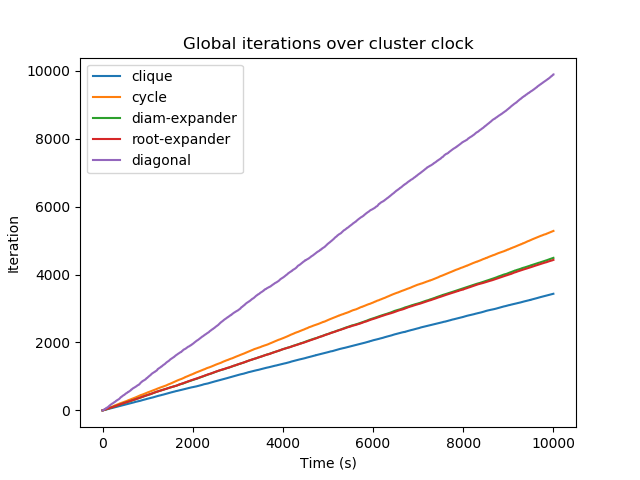
\includegraphics{media/img/tests/test_003_100samples_classic/1_iter_time.png}
This trend will be a constant through all future tests: the less the
nodes' connections the fastest the system can advance in iterations.

As expected, in diagonal topology, since nodes never wait still and
since the mean of the time taken by each iteration is equal to 1, then
such topology always achieves an amount of iterations approximately
equal to the time of the simulation. This plot makes us notice that the
amount of iteration achieved by each topology depends, in some way, on
the graph's degree (e.g. number of dependency established among nodes).
We would like to study in depth this intuition.

    \subsubsection{100 sample GD test - MSE over
iterations}\label{sample-gd-test---mse-over-iterations}

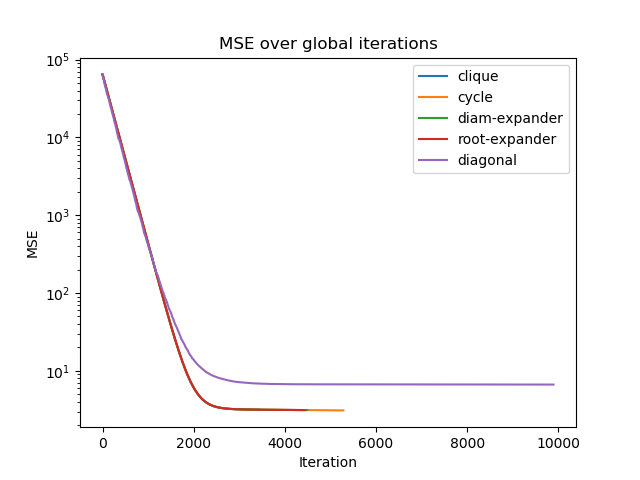
\includegraphics{media/img/tests/test_003_100samples_classic/2_mse_iter.png}
Due to restricted training set size, a single node doesn't own enough
samples to achieve a good model without communicating with other nodes,
therefore diagonal topology performs far worse than the others, which in
turn behave almost equally.

    \subsubsection{100 samples GD test - RMSE over
iterations}\label{samples-gd-test---rmse-over-iterations}

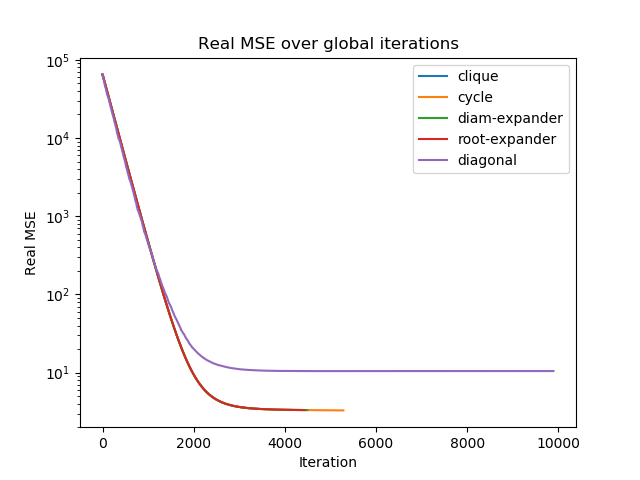
\includegraphics{media/img/tests/test_003_100samples_classic/2_real-mse_iter.png}
RMSE/iter plot doesn't suggest anything more than MSE/iter already does.

    \subsubsection{100 samples GD test - MSE over
time}\label{samples-gd-test---mse-over-time}

\begin{figure}
\centering
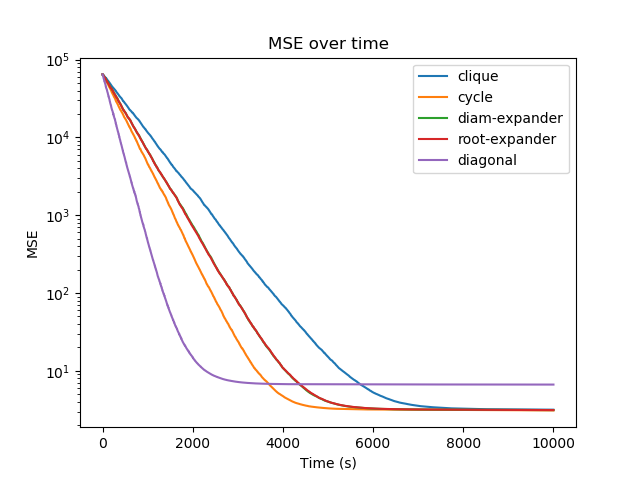
\includegraphics{media/img/tests/test_003_100samples_classic/3_mse_time.png}
\caption{MSE over time}
\end{figure}

    \subsubsection{100 samples GD test - RMSE over
time}\label{samples-gd-test---rmse-over-time}

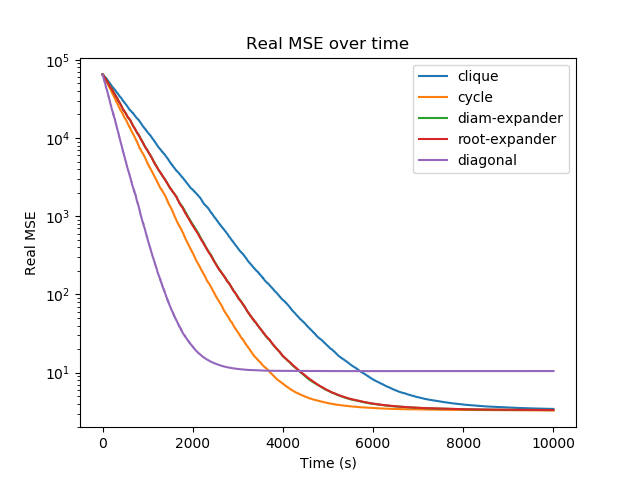
\includegraphics{media/img/tests/test_003_100samples_classic/3_real-mse_time.png}
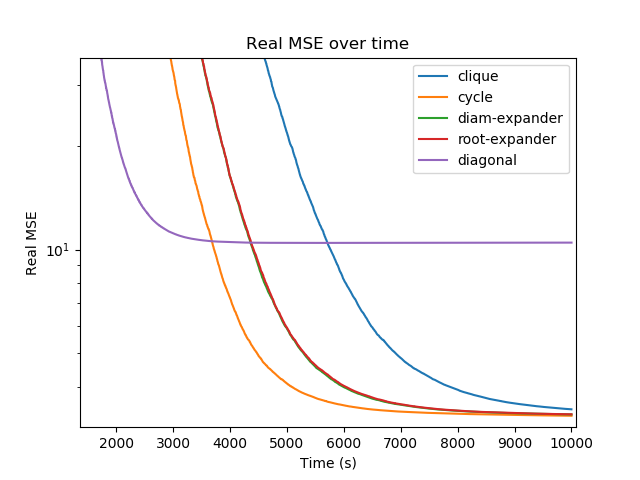
\includegraphics{media/img/tests/test_003_100samples_classic/3_real-mse_time_zoom.png}

As already seen in previous plots for this test, diagonal topology,
unlike all the others, never achieves a good prediction model.

The cycle turns out to be the fastest.

2-degree graphs plots (root expander and diameter expander) are very
close.

\emph{The same test with different seeds has led to almost identical
results.}

    \subsection{1k samples GD test}\label{k-samples-gd-test}

\texttt{n\_samples\ =\ 1000}.

    \subsubsection{1k samples GD test - iterations over
time}\label{k-samples-gd-test---iterations-over-time}

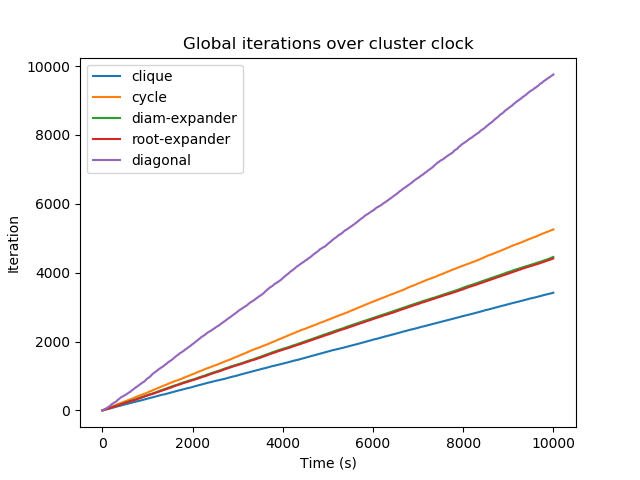
\includegraphics{media/img/tests/test_003_1ksamples_classic/1_iter_time.png}
Almost the same result as in 100 samples test.

    \subsubsection{1k samples GD test - MSE over
iterations}\label{k-samples-gd-test---mse-over-iterations}

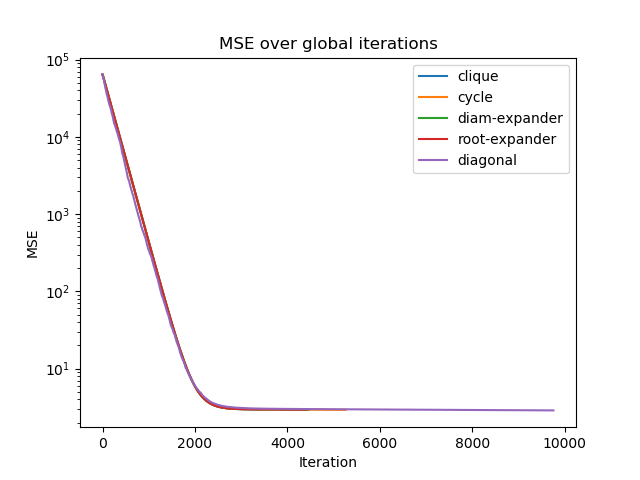
\includegraphics{media/img/tests/test_003_1ksamples_classic/2_mse_iter.png}
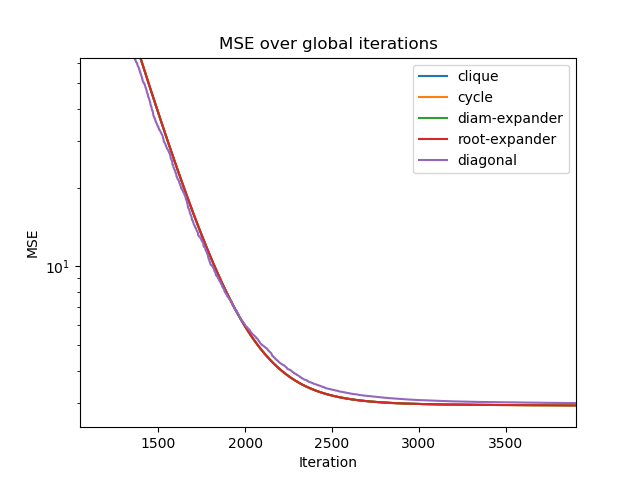
\includegraphics{media/img/tests/test_003_1ksamples_classic/2_mse_iter_zoom.png}

Now, since the amount of samples in the training set is equal to 1000,
each node \(i\) owns a subsample \(\mathcal{X}_i \subset \mathcal{X}\)
such that \(|\mathcal{X}_i| = 100\) (when for \(|\mathcal{X}|=100\),
\(|\mathcal{X}_i|=10\)). Such condition seems enough for the diagonal
topology to perform similarly as those with communications among nodes.

    \subsubsection{1k samples GD test - RMSE over
iterations}\label{k-samples-gd-test---rmse-over-iterations}

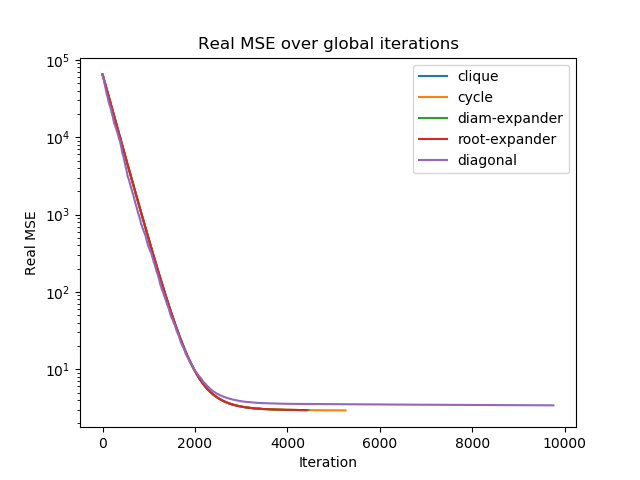
\includegraphics{media/img/tests/test_003_1ksamples_classic/2_real-mse_iter.png}
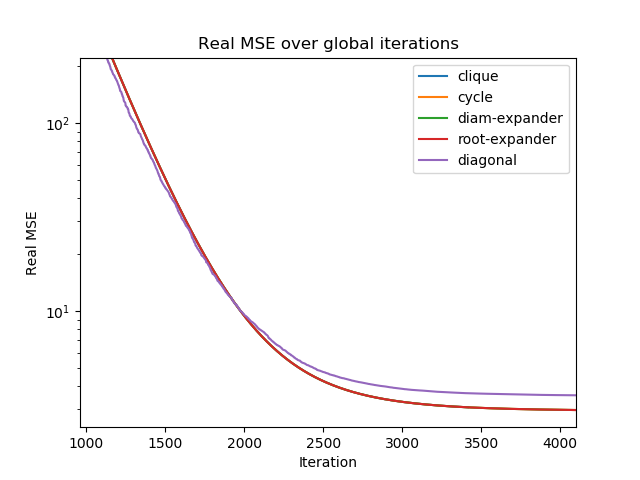
\includegraphics{media/img/tests/test_003_1ksamples_classic/2_real-mse_iter_zoom.png}
By comparing MSE/iter and RMSE/iter, we notice that diagonal topology
suffers noise more than others topologies do.

    \subsubsection{1k samples GD test - MSE over
time}\label{k-samples-gd-test---mse-over-time}

\begin{figure}
\centering
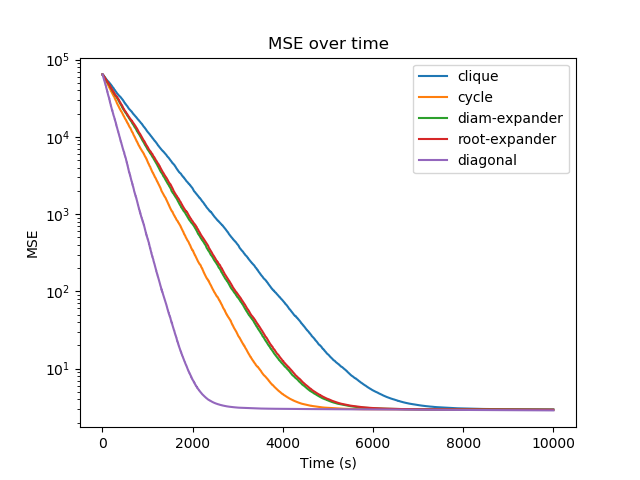
\includegraphics{media/img/tests/test_003_1ksamples_classic/3_mse_time.png}
\caption{MSE over time}
\end{figure}

    \subsubsection{1k samples GD test - RMSE over
time}\label{k-samples-gd-test---rmse-over-time}

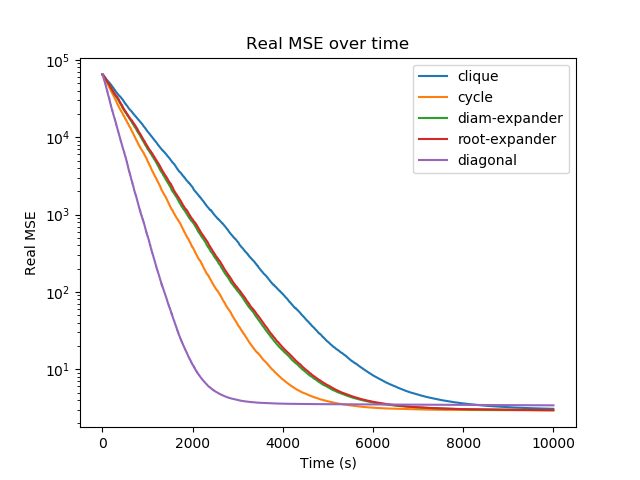
\includegraphics{media/img/tests/test_003_1ksamples_classic/3_real-mse_time.png}
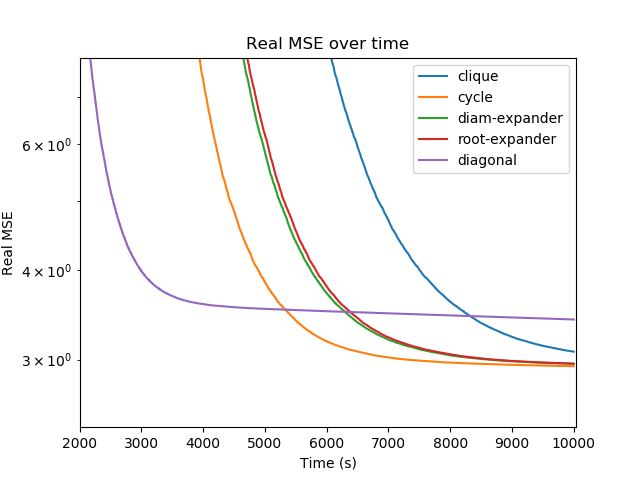
\includegraphics{media/img/tests/test_003_1ksamples_classic/3_real-mse_time_zoom.png}

Despite the behaviour of topologies, with respect to \textbf{convergence
speed}, is almost the same as the one observed in the \emph{100 samples
test MSE/time plot}, now diagonal topology doesn't behave so bad anymore
(its error differs only by 1 from other topologies).

\emph{The same test with different seeds has led to almost identical
results.}

    \subsection{10k samples test}\label{k-samples-test}

\texttt{n\_samples\ =\ 10000}.

    \subsubsection{10k samples GD test - iterations over
time}\label{k-samples-gd-test---iterations-over-time}

\begin{figure}
\centering
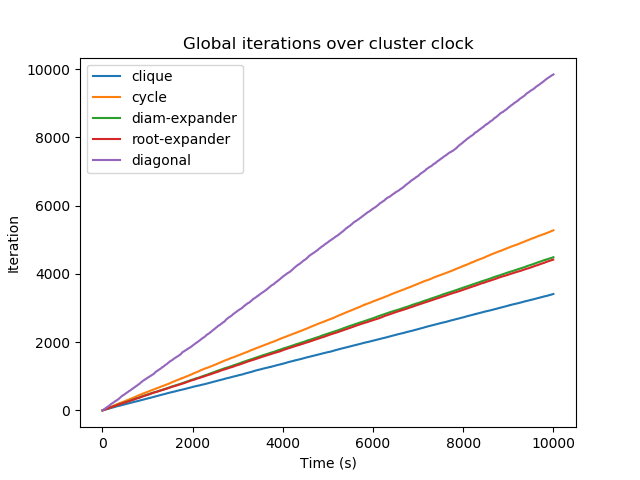
\includegraphics{media/img/tests/test_003_10ksamples_classic/1_iter_time.png}
\caption{Iterations over time}
\end{figure}

    \subsubsection{10k samples GD test - MSE over
iterations}\label{k-samples-gd-test---mse-over-iterations}

\begin{figure}
\centering
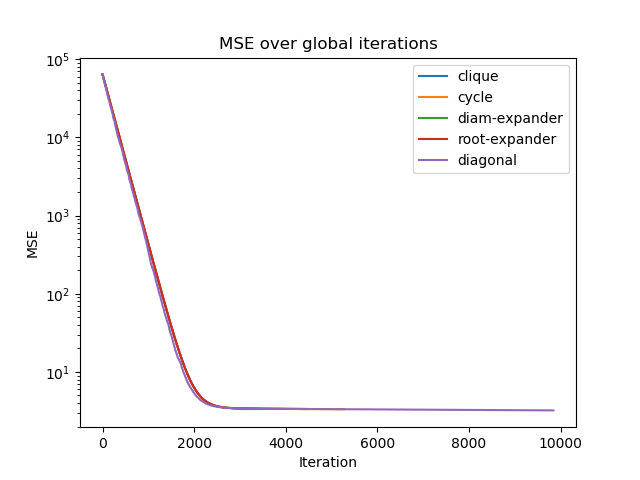
\includegraphics{media/img/tests/test_003_10ksamples_classic/2_mse_iter.png}
\caption{MSE over iterations}
\end{figure}

    \subsubsection{10k samples GD test - RMSE over
iterations}\label{k-samples-gd-test---rmse-over-iterations}

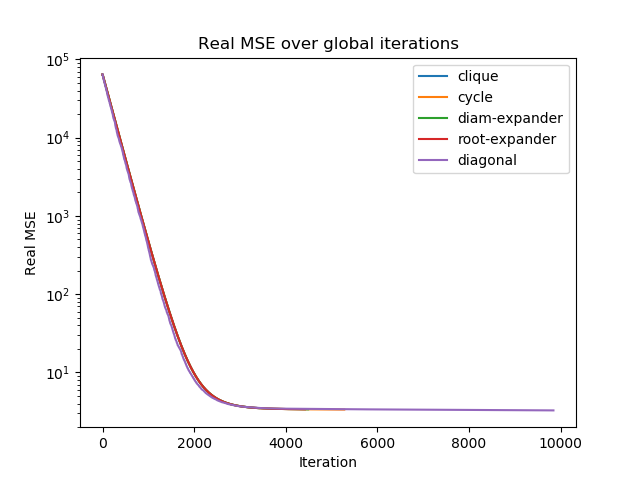
\includegraphics{media/img/tests/test_003_10ksamples_classic/2_real-mse_iter.png}
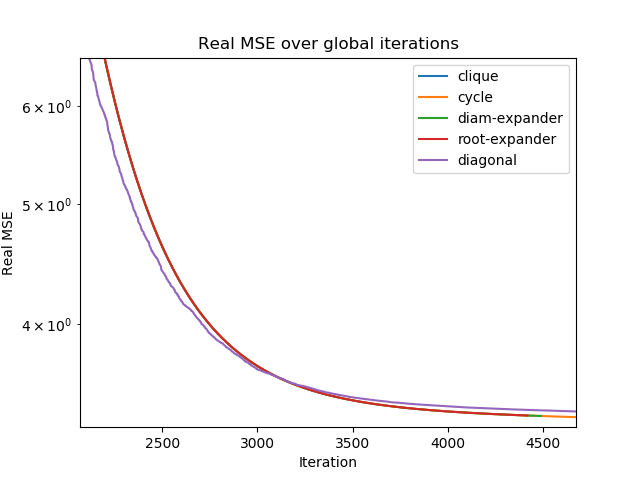
\includegraphics{media/img/tests/test_003_10ksamples_classic/2_real-mse_iter_zoom.png}

    \subsubsection{10k samples GD test - MSE over
time}\label{k-samples-gd-test---mse-over-time}

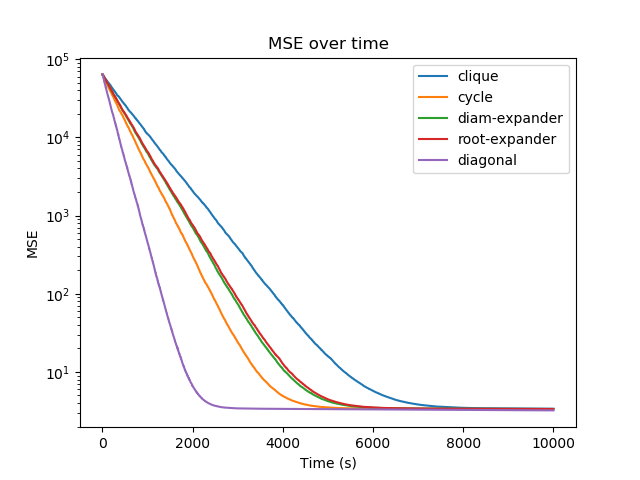
\includegraphics{media/img/tests/test_003_10ksamples_classic/3_mse_time.png}
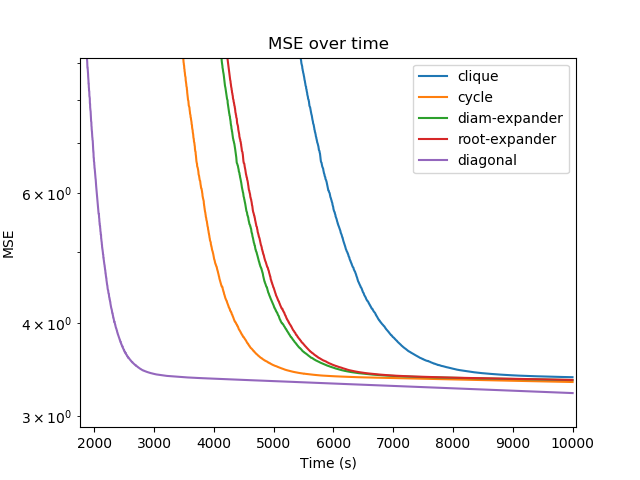
\includegraphics{media/img/tests/test_003_10ksamples_classic/3_mse_time_zoom.png}

    \subsubsection{10k samples GD test - RMSE over
time}\label{k-samples-gd-test---rmse-over-time}

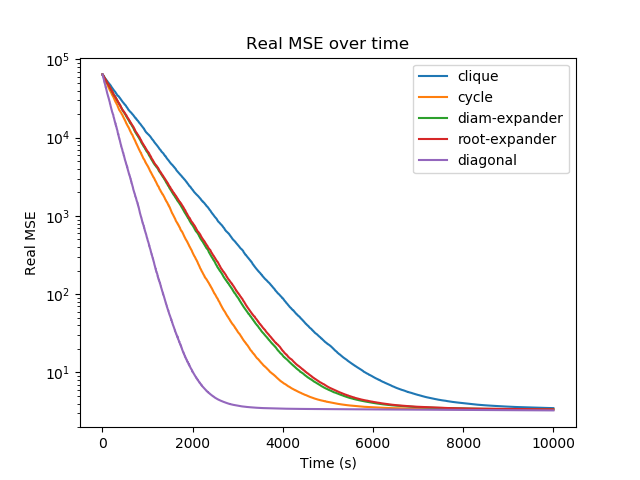
\includegraphics{media/img/tests/test_003_10ksamples_classic/3_real-mse_time.png}
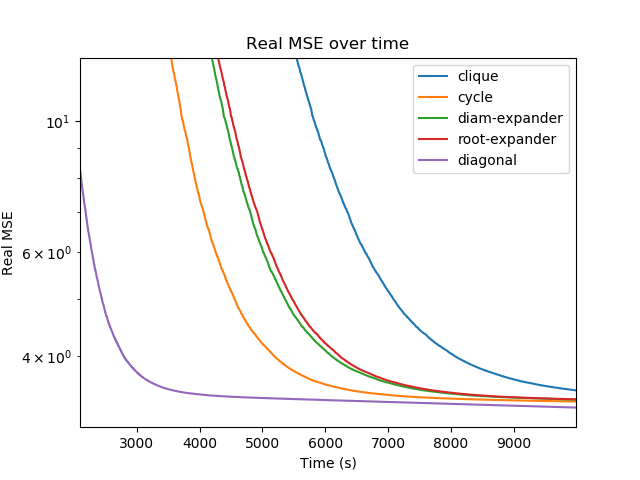
\includegraphics{media/img/tests/test_003_10ksamples_classic/3_real-mse_time_zoom.png}

With \(10000\) samples diagonal outperforms others topologies with
regard to either MSE/time and RMSE/time plots.

\emph{The same test with different seeds has led to almost identical
results.}

    \subsection{100k samples GD test}\label{k-samples-gd-test}

\texttt{n\_samples\ =\ 100000}.

    \subsubsection{100k samples GD test - iterations over
time}\label{k-samples-gd-test---iterations-over-time}

\begin{figure}
\centering
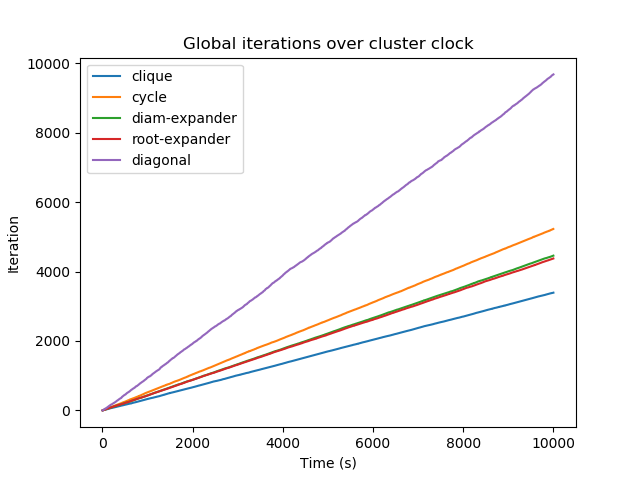
\includegraphics{media/img/tests/test_003_100ksamples_classic/1_iter_time.png}
\caption{Iterations over time}
\end{figure}

    \subsubsection{100k samples GD test - MSE over
iterations}\label{k-samples-gd-test---mse-over-iterations}

\begin{figure}
\centering
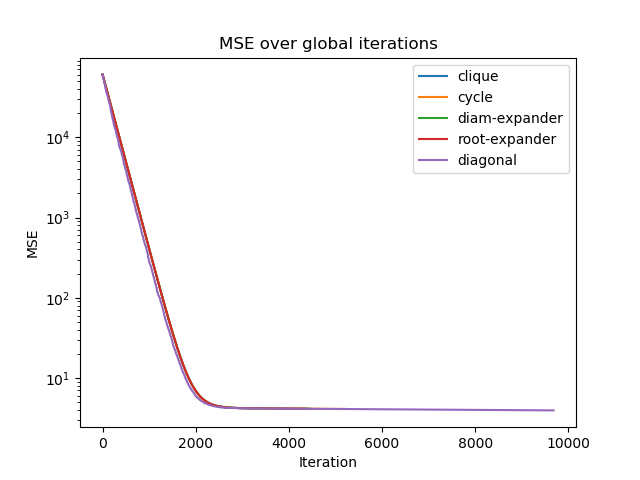
\includegraphics{media/img/tests/test_003_100ksamples_classic/2_mse_iter.png}
\caption{MSE over iterations}
\end{figure}

    \subsubsection{100k samples GD test - RMSE over
iterations}\label{k-samples-gd-test---rmse-over-iterations}

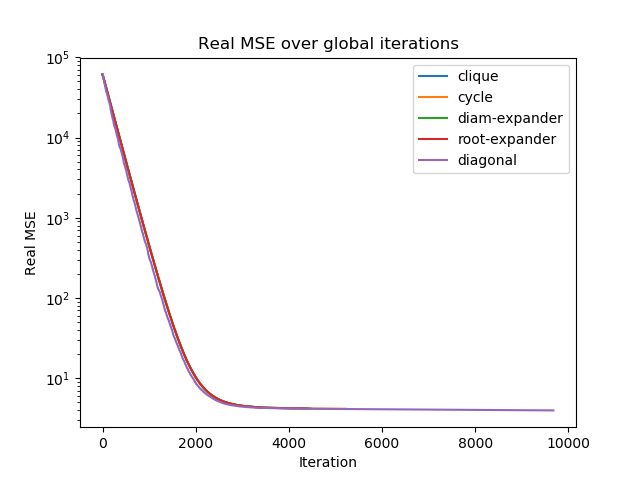
\includegraphics{media/img/tests/test_003_100ksamples_classic/2_real-mse_iter.png}
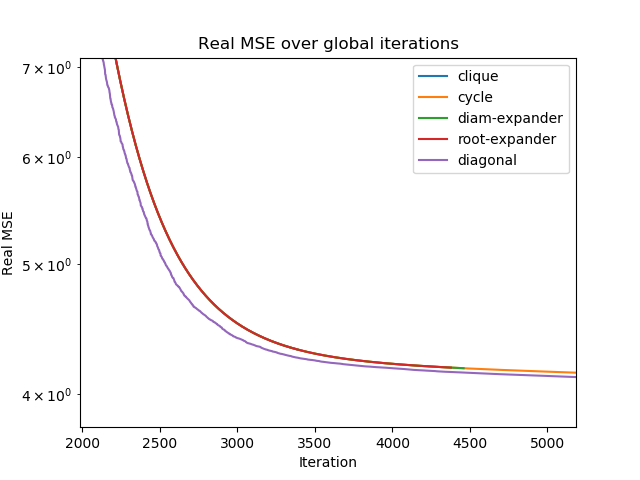
\includegraphics{media/img/tests/test_003_100ksamples_classic/2_real-mse_iter_zoom.png}

    \subsubsection{100k samples GD test - MSE over
time}\label{k-samples-gd-test---mse-over-time}

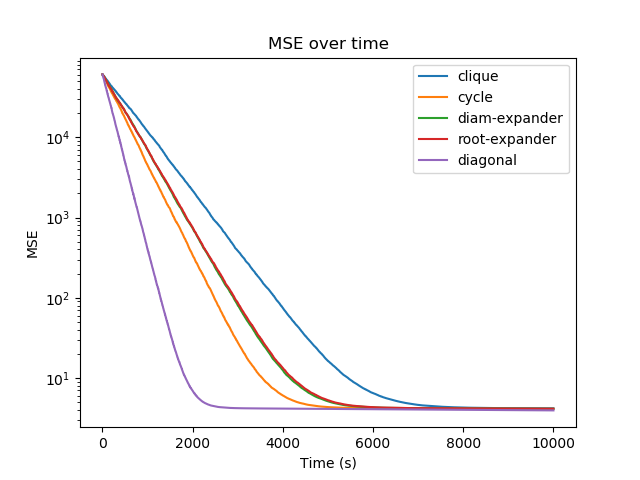
\includegraphics{media/img/tests/test_003_100ksamples_classic/3_mse_time.png}
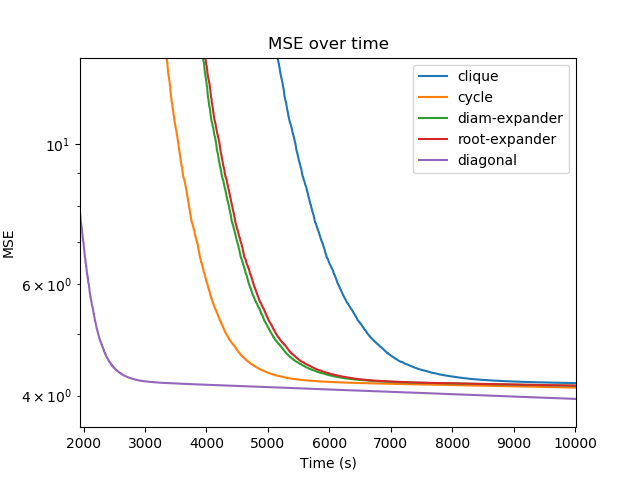
\includegraphics{media/img/tests/test_003_100ksamples_classic/3_mse_time_zoom.png}

    \subsubsection{100k samples GD test - RMSE over
time}\label{k-samples-gd-test---rmse-over-time}

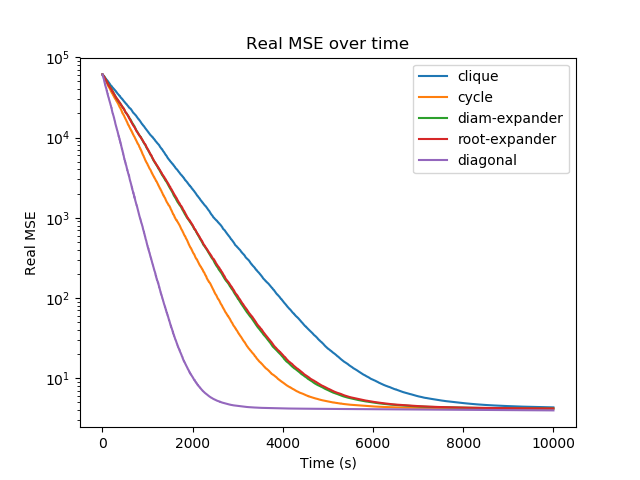
\includegraphics{media/img/tests/test_003_100ksamples_classic/3_real-mse_time.png}
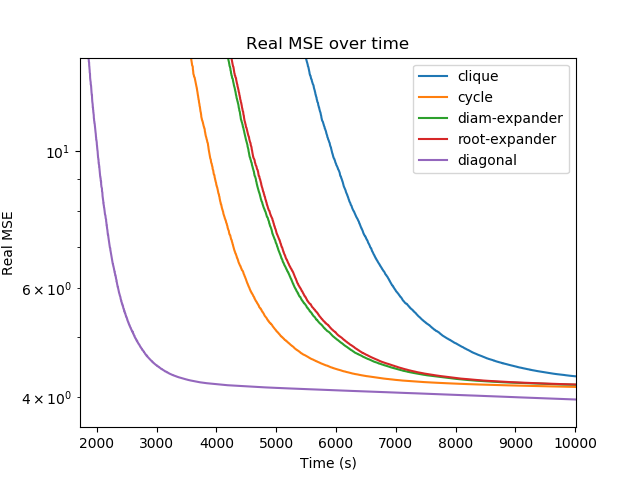
\includegraphics{media/img/tests/test_003_100ksamples_classic/3_real-mse_time_zoom.png}

\emph{The same test with different seeds has led to almost identical
results.}

    While the training set gets bigger, diagonal topology turns out to be by
far the fastest. I would like to make some tests with different kinds of
training sets to assess whether this results are strongly related to
this training set morphology or can be extended to more general cases.

    \begin{center}\rule{0.5\linewidth}{\linethickness}\end{center}

Below tests with 100 and 1000 samples repeated with
\texttt{method=\textquotesingle{}stochastic\textquotesingle{}} instead
of \texttt{classic} for the gradient descent.

\subsection{100 samples SGD test}\label{samples-sgd-test}

\subsubsection{100 samples SGD test - iterations over
time}\label{samples-sgd-test---iterations-over-time}

\begin{figure}
\centering
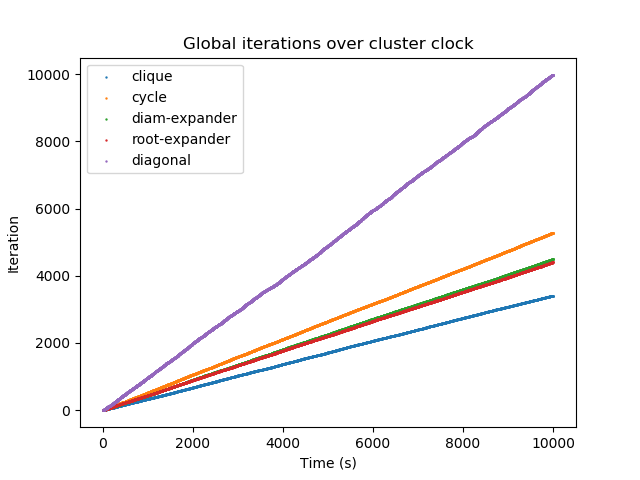
\includegraphics{media/img/tests/test_003_100samples_stochastic/1_iter_time.png}
\caption{Iterations over time}
\end{figure}

\subsubsection{100 samples SGD test - MSE over
iterations}\label{samples-sgd-test---mse-over-iterations}

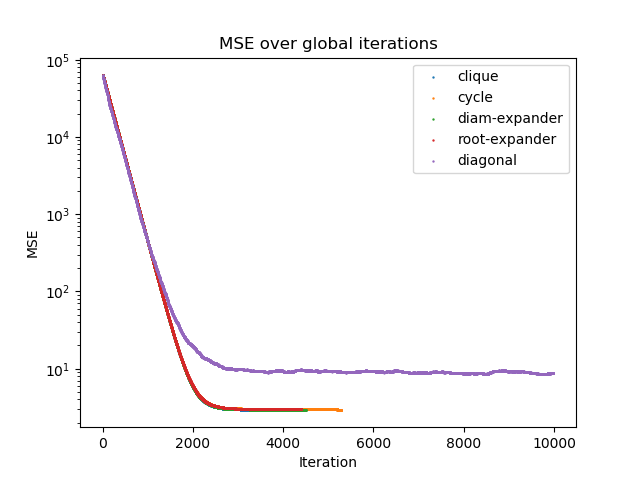
\includegraphics{media/img/tests/test_003_100samples_stochastic/2_mse_iter.png}
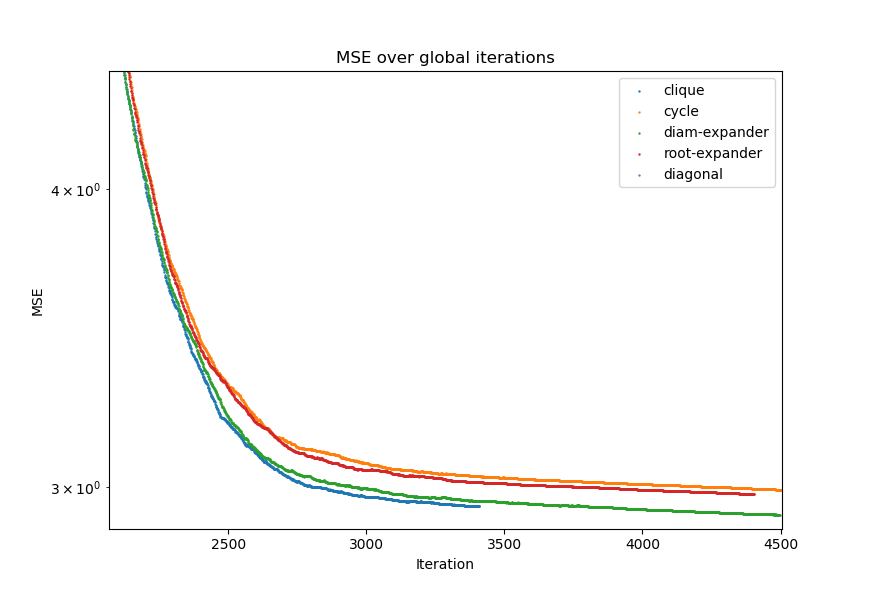
\includegraphics{media/img/tests/test_003_100samples_stochastic/2_mse_iter_zoom.png}

\subsubsection{100 samples SGD test - RMSE over
iterations}\label{samples-sgd-test---rmse-over-iterations}

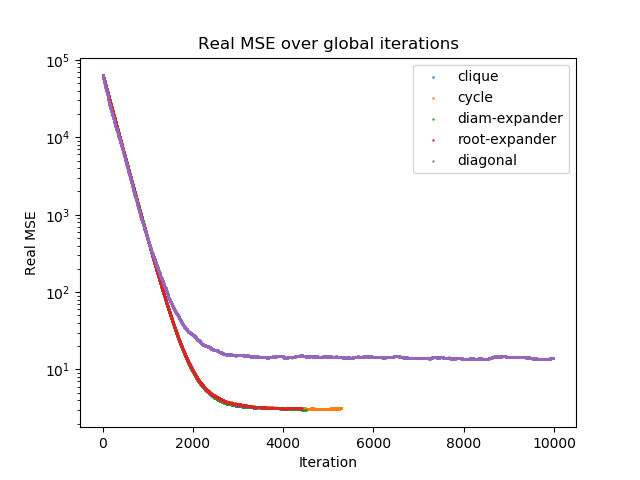
\includegraphics{media/img/tests/test_003_100samples_stochastic/2_real-mse_iter.png}
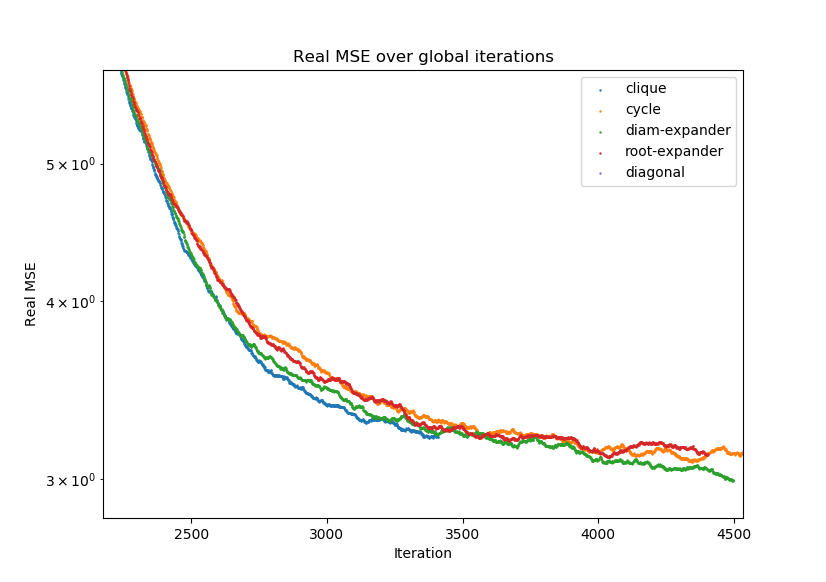
\includegraphics{media/img/tests/test_003_100samples_stochastic/2_real-mse_iter_zoom.png}

\subsubsection{100 samples SGD test - MSE over
time}\label{samples-sgd-test---mse-over-time}

\begin{figure}
\centering
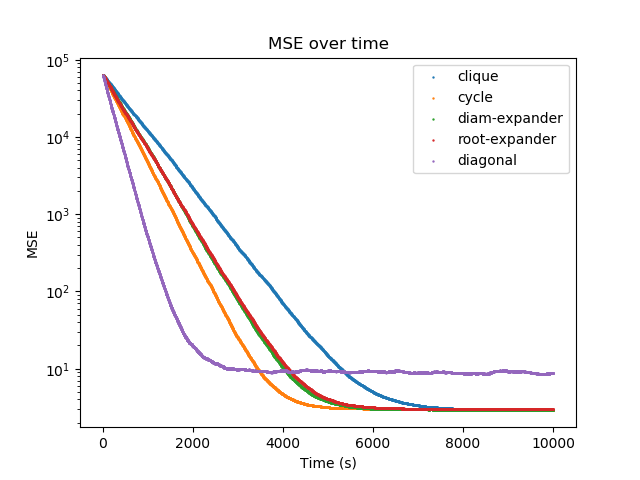
\includegraphics{media/img/tests/test_003_100samples_stochastic/3_mse_time.png}
\caption{MSE over time}
\end{figure}

\subsubsection{100 samples SGD test - RMSE over
time}\label{samples-sgd-test---rmse-over-time}

\begin{figure}
\centering
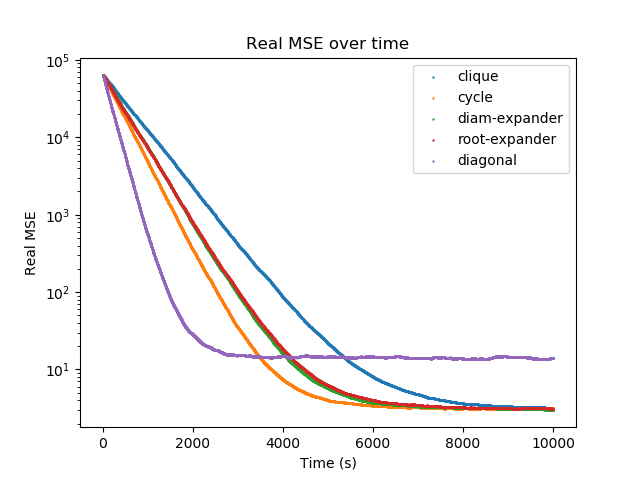
\includegraphics{media/img/tests/test_003_100samples_stochastic/3_real-mse_time.png}
\caption{RMSE over time}
\end{figure}

    \subsection{1k samples SGD test}\label{k-samples-sgd-test}

\subsubsection{1k samples SGD test - iterations over
time}\label{k-samples-sgd-test---iterations-over-time}

\begin{figure}
\centering
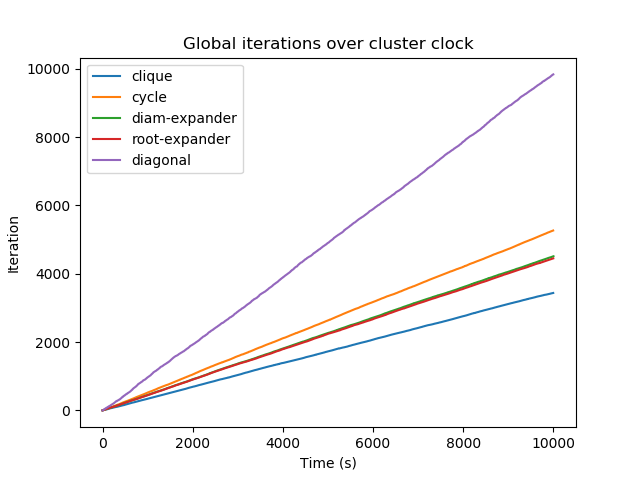
\includegraphics{media/img/tests/test_003_1ksamples_stochastic/1_iter_time.png}
\caption{Iterations over time}
\end{figure}

\subsubsection{1k samples SGD test - MSE over
iterations}\label{k-samples-sgd-test---mse-over-iterations}

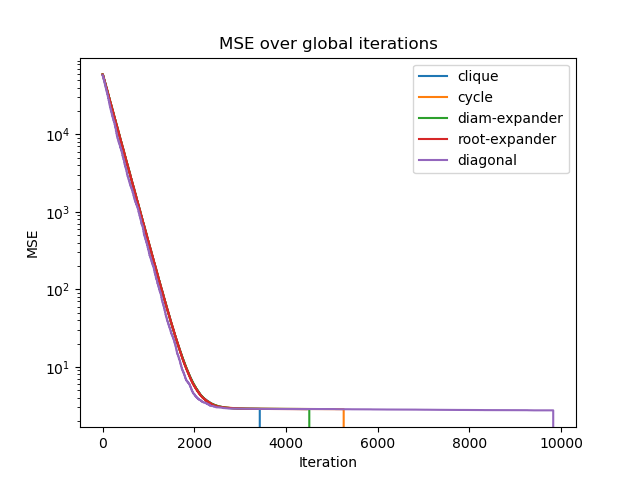
\includegraphics{media/img/tests/test_003_1ksamples_stochastic/2_mse_iter.png}
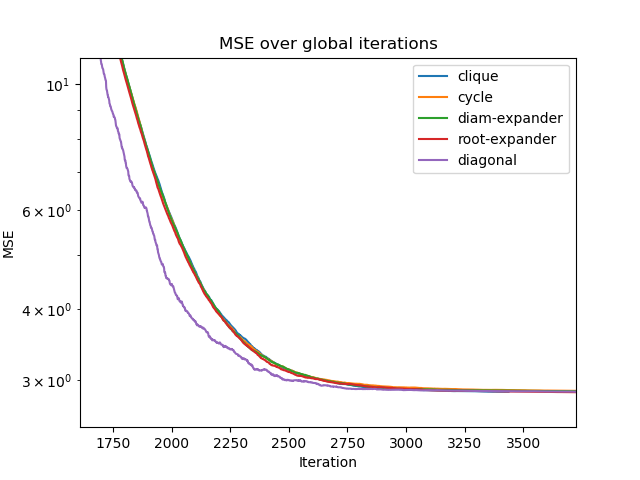
\includegraphics{media/img/tests/test_003_1ksamples_stochastic/2_mse_iter_zoom.png}

\subsubsection{1k samples SGD test - RMSE over
iterations}\label{k-samples-sgd-test---rmse-over-iterations}

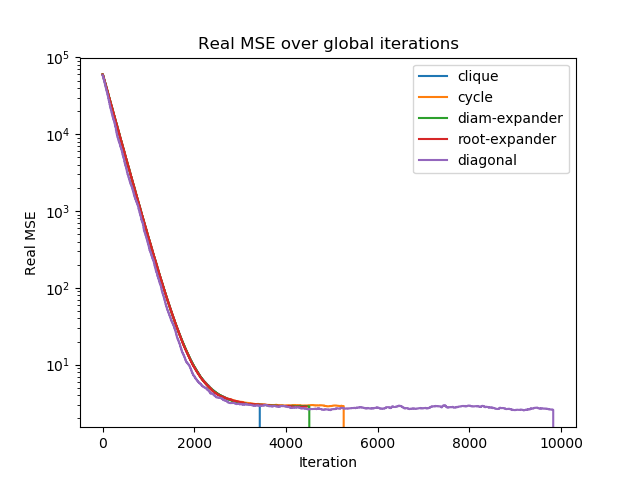
\includegraphics{media/img/tests/test_003_1ksamples_stochastic/2_real-mse_iter.png}
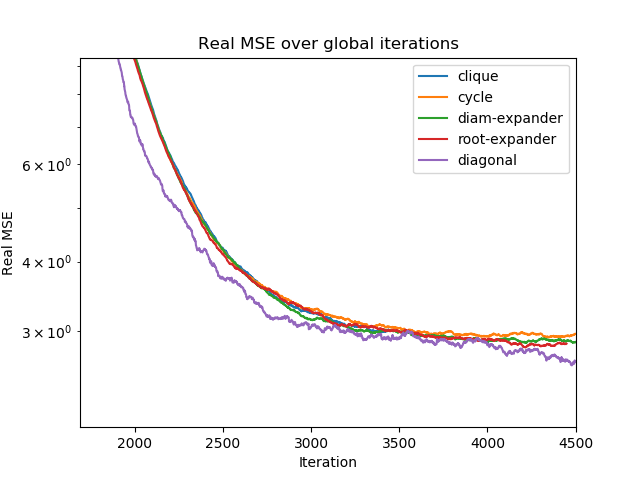
\includegraphics{media/img/tests/test_003_1ksamples_stochastic/2_real-mse_iter_zoom.png}

\subsubsection{1k samples SGD test - MSE over
time}\label{k-samples-sgd-test---mse-over-time}

\begin{figure}
\centering
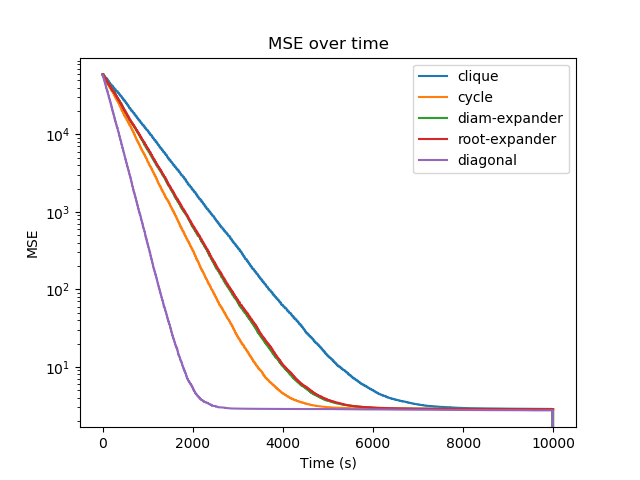
\includegraphics{media/img/tests/test_003_1ksamples_stochastic/3_mse_time.png}
\caption{MSE over time}
\end{figure}

\subsubsection{1k samples SGD test - RMSE over
time}\label{k-samples-sgd-test---rmse-over-time}

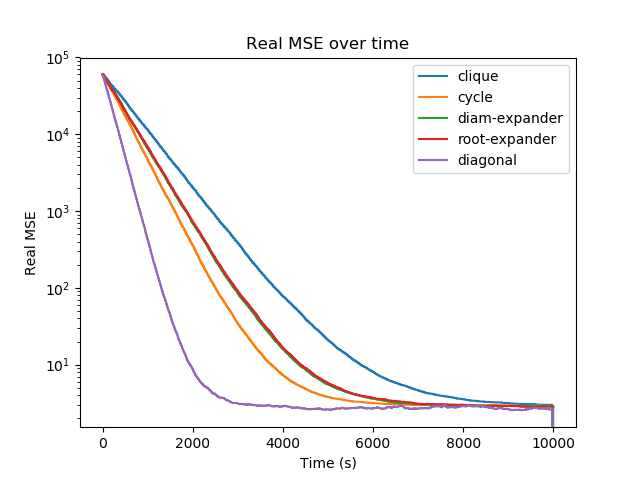
\includegraphics{media/img/tests/test_003_1ksamples_stochastic/3_real-mse_time.png}
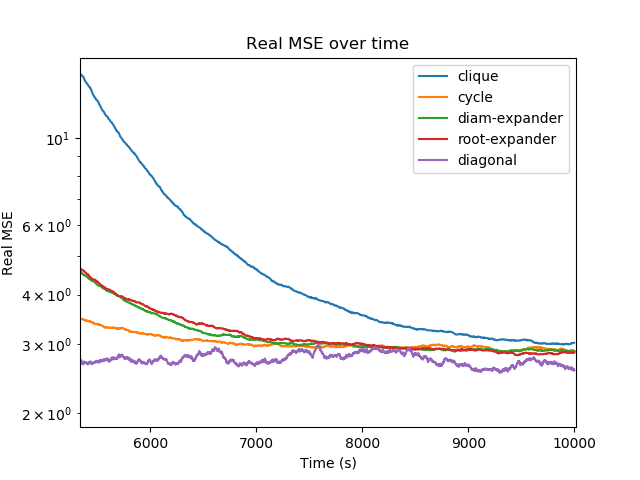
\includegraphics{media/img/tests/test_003_1ksamples_stochastic/3_real-mse_time_zoom.png}

    \subsection{Theoretical point of view}\label{theoretical-point-of-view}

\subsubsection{Nodes' degree}\label{nodes-degree}

We've noticed that the iterations' speed is strongly related to the
number of connections established among nodes, this is clearly
observable in all \emph{iteration over time} plots. A similar speed gain
can be seen in \emph{MSE over time} plot: whether the amount of samples
in the training set is big enough such that even a single node alone can
achieve a good solution, then connections are just cause of slowdown. It
seems that the gain in iterations' speed always matters far more than
the gain in information flow due to an high dependency graph's degree.
This is only a suggestion given by these early tests.

Consider the following plot (\emph{MSE over time 10k samples GD test
003}).

\begin{figure}
\centering
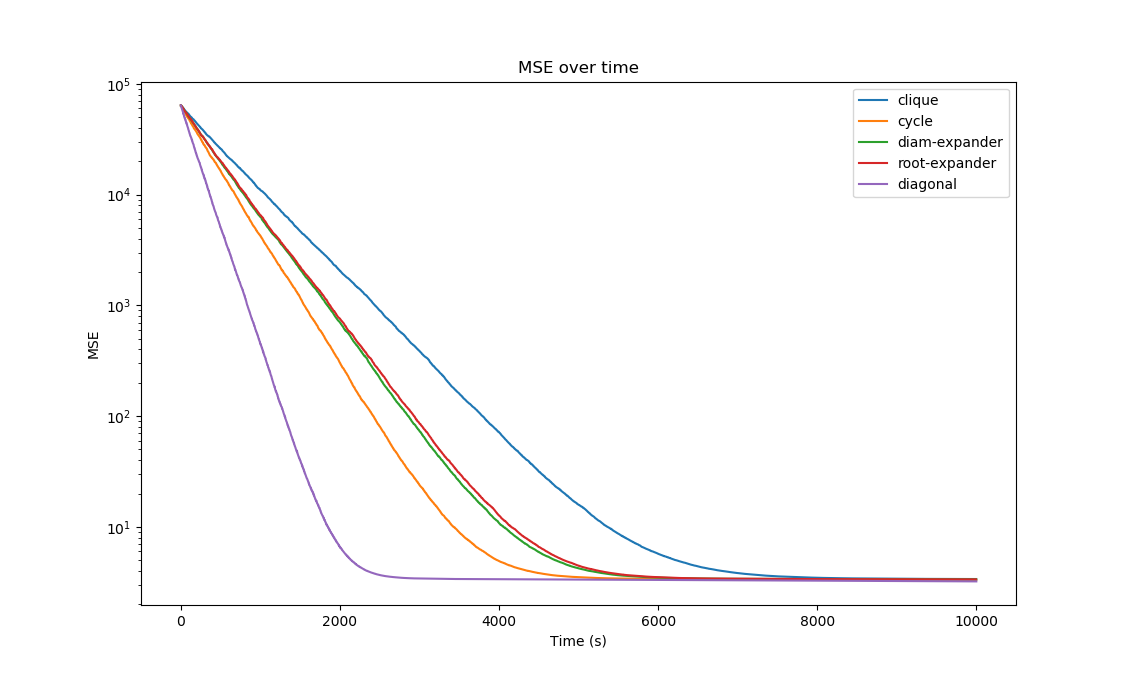
\includegraphics{media/img/tests/test_003_10ksamples_classic/3_mse_time_big.png}
\caption{MSE\_over\_time}
\end{figure}

By inverting it we obtain the plot below. \emph{NB: actually such
functions aren't invertible since in small intervals the error can
oscillate, anyway fixes can be applied to make them invertible (like
exploiting a moving average).}

\begin{figure}
\centering
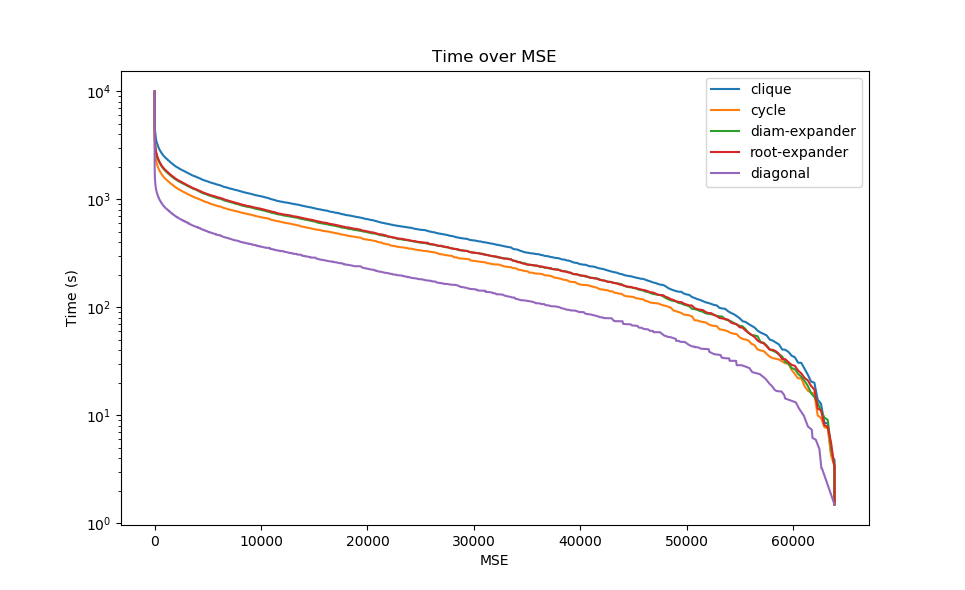
\includegraphics{media/img/tests/test_003_10ksamples_classic/4_time_mse_big.png}
\caption{Time over MSE}
\end{figure}

We can compare the time taken by each topology to achieve a same value
of MSE, then effectively estimate the speed ratio among different
topologies. The same will be done for RMSE/time, MSE/iter and RMSE/iter
plots too.

    \subsubsection{Dependency graph's
diameter}\label{dependency-graphs-diameter}

Assume all nodes in the system being at iteration \(r>0\), assume that
one node \(s\) gets stuck there (it never advances to iteration
\(r+1\)), then: - nodes at distance 1 from \(s\) can advance only by one
more iteration; - nodes at distance 2 from \(s\) can advance only by two
more iterations; - and so on, up to nodes at distance \(d_s\) from \(s\)
(where \(d_s = max\{dist(s, i) : i \in V\}\)) that can advance by
\(d_s\) more iterations.

In general: \[
\forall i,j \in V,\ i \text{ is at iteration }r \Rightarrow j \text{ is at iteration } \in [r-dist(i,j),r+dist(i,j)] \subseteq \mathbb{N}.
\]

Since \(\forall i,j \in V,\ dist(i,j) \leq diam\) (where \(diam\) is the
graph's diameter), then the maximum distance between two nodes, with
respect to iterations' number, is always less than or equal to the graph
diameter. Even this property seems to be a key factor in speed gain.

For instance, the following inequality
\[diam(\text{clique}) = 1 < diam(\text{diam-expander}) = \frac{n}{2} < diam(\text{cycle}) = n-1\]
holds also for the speed: the cycle is faster than the diam-expander
which in turn is faster than the clique.

The questions now I am looking an answer for are: 1. how the speed is
related to the nodes' degree? 2. how the speed is related to graph's
diameter? 3. how much do degree and diameter weight in the observed
topologies' speed? which matters more?

    \subsubsection{System dynamic}\label{system-dynamic}

Let \(r \geq 0\) be a fixed iteration number. Let \(X_1, X_2, ..., X_n\)
be \(n\) independent random variables where \(X_i\) is the time taken by
node \(i\) to advance to iteration \(r+1\). At the moment we consider
\(X_i \sim Exp(\lambda = 1)\), so -
\(P(X_i \leq t) = 1-e^{-\lambda t} = 1-e^{-t}\), hence
\(P(X_i > t) = e^{-\lambda t} = e^{-t}\). -
\(\mathbb{E}[X_i] = \frac{1}{\lambda} = 1\).

Lets define a new random variable \(Z = max\{X_i : 1 \leq i \leq n\}\).
\(Z\) is the time taken by the slowest node to complete the \((r+1)\)-th
update of its weight vector, where: -
\(P(Z \leq z) = \prod_{i=1}^{n} P(X_i \leq z) = (1-e^{-t})^n\); -
\(\mathbb{E}[Z] = \prod_{i=1}^{n} \mathbb{E}[X_i] = (\frac{1}{\lambda})^n = 1\).

\(Z\) reflects the time taken by the slowest node to perform the
\((r+1)\)-th weight update.

It is easy to exploit \(Z\) to analyze the clique behaviour since \(Z\)
is exactly the time taken by each node to perform the \((r+1)\)-th
update of its weight. For other topologies it is not so trivial. Anyway,
this is the way I will follow to give significance from a theoretical
point of view to results.


    % Add a bibliography block to the postdoc
    
    
    
    \end{document}
